%% LyX 1.3 created this file.  For more info, see http://www.lyx.org/.
%% Do not edit unless you really know what you are doing.
\documentclass[english,useAMS, usenatbib]{mn2e}
\usepackage[T1]{fontenc}
\usepackage[latin1]{inputenc}
\usepackage{times}
\usepackage{graphicx}
\usepackage{amssymb}

\setcounter{tocdepth}{3}
\makeatletter

%%%%%%%%%%%%%%%%%%%%%%%%%%%%%% LyX specific LaTeX commands.
%% Bold symbol macro for standard LaTeX users
\newcommand{\boldsymbol}[1]{\mbox{\boldmath $#1$}}

%% Because html converters don't know tabularnewline
\providecommand{\tabularnewline}{\\}

%%%%%%%%%%%%%%%%%%%%%%%%%%%%%% User specified LaTeX commands.

\newcommand{\aap}{A\&A}
\newcommand{\aaps}{A\&AS}
\newcommand{\apj}{ApJ}
\newcommand{\apjl}{\apj}
\newcommand{\pasp}{PASP}
\newcommand{\aj}{AJ}
\newcommand{\mnras}{MNRAS}
\newcommand{\apjs}{ApJS}
\newcommand{\aapr}{A\&AR}
\newcommand{\pasj}{PASJ}

\newcommand{\kmps}{\mathrm{km~s^{-1}}}
\newcommand\ion[2]{#1$\,${\sc {#2}}}   % ion, i.e., CII = \ion{C}{ii}
\newcommand{\Kelvin}{\mathrm{K}}

\usepackage{babel}
\makeatother
\begin{document}
\title[On the formation of H$\alpha$ around classical T Tauri
  stars]{On the formation of H$\alpha$ line emission around classical T Tauri stars}

\author[R. Kurosawa et\,al.]{Ryuichi
  Kurosawa$^1$\thanks{E-mail:rk@astro.ex.ac.uk}, Tim J. Harries$^1$
  and Neil H. Symington$^2$\\ $^1$School of Physics, University of Exeter, Stocker Road, Exeter EX4~4QL. \\ $^2$School of Physics and Astronomy, University of St. Andrews, North Haugh, St. Andrews, Fife, KY16 9SS.}

\date{Dates to be inserted}

\pagerange{\pageref{firstpage}--\pageref{lastpage}} \pubyear{2005}

\maketitle

\label{firstpage}

\begin{abstract}

We present radiative transfer models of the circumstellar environment
of classical T~Tauri stars, concentrating on the formation of the
H$\alpha$ emission. The wide variety of line profiles seen in
observations are indicative of both inflow and outflow, and we
therefore employ a circumstellar structure that includes both
magnetospheric accretion and a wind. We adopt two kinematic models for
the outflow, a generic bipolar wind and a disc wind. We perform
systematic investigations of the model parameters for the wind and the
magnetosphere to search for possible geometrical and physical
conditions which lead to the types of profiles seen in
observations. We find that both wind models can reproduce the wide
range profile types seen is observations, and that the most common
profile types observed occupy a large volume of parameter
space. Conversely, the most infrequently observed profile morphologies
require a very specific set of models parameters.  Although a
particular outflow model (bipolar or disc-wind) is not
well-constrained by a single line profile observations, we find that
the inclination dependence of the line equivalent width predicted by
the bipolar wind model agree with trends seen in the observation, but
the disc-wind model does not. Using the model results, we examine the
H$\alpha$ spectroscopic classification used by Reipurth et.~al, and
discuss the basic physical conditions that are required to reproduce
the profiles in each classified type.

\end{abstract}

\begin{keywords}
stars: formation -- circumstellar matter -- radiative transfer -- stars: pre-main-sequence
\end{keywords}


\section{Introduction }

\label{sec:Introduction}

T~Tauri stars (TTS) are young ($\gtrsim 3\times10^{6}\,\mathrm{yrs}$,
\citealt{appenzeller:1989}) low-mass objects, and are the progenitors
of solar-type stars. Classical T~Tauri stars (CTTS) exhibit strong
H$\alpha$ emission, and typically have spectral types of F--K. Some of
the most active CTTS show emission in higher Balmer lines and metal
lines (e.g., \ion{Ca}{ii}~H and K). They also exhibit excess continuum
flux in the ultraviolet (UV) and infrared (IR).  Their spectral energy
distribution and polarisation data suggest the presence of
circumstellar discs, which plays an important role in regulating
dynamics of gas flows around CTTS (e.g. \citealt{camenzind:1990}).

Many observational studies (e.g., \citealt{herbig:1962};
\citealt{edwards:1994}; \citealt{kenyon:1994};
\citealt*{reipurth:1996}; \citealt{alencar:2000}) of CTTS line
profiles have revealed evidence for both outward wind flows and inward
accretion flows, characterised by the blue-shifted absorption features
in H$\alpha$ profiles and the redshifted inverse P~Cygni (IPC)
profiles respectively. Typical mass-loss rates of CTTS are about
$10^{-9}\,\mathrm{M_{\sun}\, yr^{-1}}$ to $10^{-7}\,\mathrm{M_{\sun}\,
yr^{-1}}$ (e.g., \citealt{kuhi:1964}; \citealt{edwards:1987};
\citealt*{hartigan:1995}), and the mass-accretion rates are also about
$10^{-9}\,\mathrm{M_{\sun}\, yr^{-1}}$ to $10^{-7}\,\mathrm{M_{\sun}\,
yr^{-1}}$ (e.g., \citealt{kenyon:1987}; \citealt*{bertout:1988};
\citealt{gullbring:1998}).  Recent H$\alpha$ spectro-astrometric
observations by \citet*{takami:2003} provide indirect evidence for the
presence of bipolar and monopolar outflows down to $\sim
1\,\mathrm{au}$ scale (e.g.\,CS~Cha and RU~Lup).  Similarly, ESO VLT
observations using high-resolution ($R=50\,000$) two-dimensional
spectra of edge-on CTTS (HH30$^{*}$, HK~Tau~B, and HV~Tau~C) by
\citet{appenzeller:2005} show extended H$\alpha$ emission in the
direction perpendicular to the obscuring circumstellar disc,
suggesting the presence of the bipolar outflows. On an even larger
scale, \emph{HST} observations of HH30 \citep{burrows:1996} trace the
jet to within $\lesssim30$~au of the star. The jet has a cone shape
with an opening angle of $3^{\circ}$ between 70 and 700 au
\citep{koenigl:2000}. \citet{alencar:2000} found about 80 per cent of
their sample (30 CTTS) show blue-shifted absorption components in at
least one of the Balmer lines and Ca~K.

In the currently favoured model of accretion in CTTS, the accretion
disc is disrupted by the magnetosphere, which channels the gas from
the disc onto the stellar surface (e.g., \citealt{uchida:1985};
\citealt{koenigl:1991}; \citealt{cameron:1993};
\citealt{shu:1994}). This picture is supported by recent measurements
of strong ($\sim 10^{3}\mathrm{G}$) magnetic fields in CTTS (e.g.,
\citealt{johns-krull:1999}; \citealt{symington:2005b}) and by
radiative transfer models which reproduce the gross characteristics of
observed profiles for some TTS (\citealt*{muzerolle:2001}). In
particular the magnetospheric accretion (MA) model explains blue-ward
asymmetric emission line profiles as resulting from the partial
occultation of the flow by the stellar photosphere, while inverse
P~Cygni profiles in the MA model result from inflowing material at
near free-fall velocities seen projected against hotspots on the
stellar surface.

Despite these successes, the overwhelming observational evidence for
outflow in the CTTS suggests that the MA model is only one component
of a complex circumstellar environment. Clearly, one must include the
contribution of any wind/jet flow if one wishes to both accurately
predict the mass-accretion rate and also determined the mass-loss rate
of CTTS via emission profile modelling. The first attempt in this
direction was made by \citet{alencar:2005} who demonstrated that the
observed H$\alpha$, H$\beta$ and Na~D lines of RW Aur are better
reproduced by the radiative transfer model which included a collimated
disc-wind arising from near the inner edge of the accretion disc.


%Prior to the MA paradigm, many alternative models had
%been considered to explain the observed spectroscopic features mentioned
%above. For example, (1)~an Alfv\'{e}n wave-driven wind model
%(e.g.~\citealt{decampli:1981}; \citealt*{hartmann:1982}), (2)~a turbulent
%boundary layer (between the accretion disc and stellar surface) model
%(e.g.~\citealt{bertout:1988}; \citealt{basri:1989}), (3)~a chromospheric
%model (e.g.~\citealt*{calvet:1984}), and (4)~a disc wind model (e.g.
%\citealt*{calvet:1992b}; \citealt{kwan:1995}).  



The main aim of this paper is to find a simple kinematic model which
can reproduce the wide variety of the observed profiles, and to
perform empirical studies of line formation in an attempt to place
morphological classification schemes on a firmer physical footing. We
will also discuss whether our model is consistent with some
predictions made by recent MHD studies i.e.~
$\mu=\dot{M}_{\mathrm{wind}}/\dot{M}_{\mathrm{acc}}\approx0.1$
(e.g.~\citealt{koenigl:2000}).

In section~\ref{sec:model-configuration}, the model assumptions, and
the basic model configurations are presented. We discuss the radiative
transfer model used to compute the profiles in
section~\ref{sec:radiative-transfer-model}, and the results of model
calculations are given in section~\ref{sec:Results}.  We discuss our
results in the context of Reipurth's classification scheme in
section~\ref{sec:Discussion}, and our summary and conclusions are
presented in section~\ref{sec:Conclusions}.


\section{Model configuration}

\label{sec:model-configuration}

In order to understand how the different parts of the CTTS
circumstellar environment contribute to the formation of H$\alpha$,
the model space is divided into four different regions: (1)~a central
continuum source, (2)~the magnetospheric accretion flow, (3)~the wind
outflow, and (4)~the accretion disc. Fig.~\ref{fig:config_dipolar}
depicts the relative location of the regions in the model space.  The
density is assumed to be rotationally symmetric around the
$z$-axis. The innermost radius of the magnetosphere at the equatorial
plane coincides with the the inner radius of the accretion disc. From
the innermost part of the accretion disc, the gas falls freely, moving
along the magnetic field onto the surface of the star.  In the
following subsections we describe the details of model components.

%%%%%%%%%%%%%%%%%%%%%%%%%%%%%%%%%%%%%%%%%%%%%%%%%%%%%%%%%%%%%%%%%%%
\begin{figure*}

  \begin{center}

    \includegraphics[%
      scale=0.5]{figures/overview3.eps}
    
  \end{center}

  \caption{The basic model configuration. The system consists of four
    components: (1)~the continuum source located at the origin $\left( o
    \right)$ of the cartesian coordinates $\left(x,y,z\right)$ -- the
    $y$-axis is into the paper, (2)~the magnetospheric accretion flow,
    (3)~the bipolar wind outflow, and (4)~the accretion disc. The density
    distribution is symmetric around the $z$-axis. The innermost radius of
    the magnetosphere (at the equatorial plane) coincides with the the
    inner radius of the accretion disc. From the innermost part of the
    accretion disc, the gas falls freely, moving along the magnetic field
    onto the surface of the star. The bipolar wind starts from just
    outside the largest radius 
    ($R_{\mathrm{mo}}$) of the magnetosphere (dotted line). }

  \label{fig:config_dipolar}

\end{figure*}
%%%%%%%%%%%%%%%%%%%%%%%%%%%%%%%%%%%%%%%%%%%%%%%%%%%%%%%%%%%%%%%%%%%

\subsection{The continuum source}

\label{sub:Continuum-Source}

We adopt stellar parameters of a typical
classical T~Tauri star for the central continuum source, i.e. radius
($R_{*}$), mass ($M_{*}$), and effective temperature the photosphere
($T_{\mathrm{ph}}$) are $2\, R_{\sun}$, $0.5\, M_{\sun}$, and $4000\,\mathrm{K}$
respectively. The model atmosphere of \citet{kurucz:1979} with
$T_{\mathrm{ph}}=4000\,\mathrm{K}$ and $\log g_{*}=3.5$ (cgs) defines
the photospheric contribution to the continuum flux. The
parameters are summarised in Table~\ref{tab:std_parameters}.

An additional continuum source is considered for models which includes
magnetospheric accretion: as the infalling gas approaches the stellar
surface, it decelerates in a strong shock, and is heated to $\sim
10^{6}\,\mathrm{K}$.  The X-ray radiation produced in the shock will
be absorbed by the gas locally, and re-emitted in optical and UV
radiation (\citealt{koenigl:1991}; \citealt*{hartmann:1994}). This
will create hot rings where the magnetic field intersects with the
surface. We assume that the free-falling kinetic energy is thermalized
in the radiating layer, and is re-emitted as blackbody radiation with
a single temperature. With the parameters of the magnetosphere and the
star given above (Table~\ref{tab:std_parameters}), about $8$~per~cent
of the surface is covered by the hot rings. If the mass-accretion rate
is $10^{-7}\,\mathrm{M_{\sun}\, yr^{-1}}$, the ratio of this accretion
luminosity to the photospheric luminosity is about $0.5$, and the
corresponding temperature of the hot rings is about
$6400\,\mathrm{K}$.  The continuum emission from the hot rings is
taken into account when computing the line profiles.

\begin{table*}

\caption{Summary of the reference classical T~Tauri star model parameters.}
\label{tab:std_parameters}

\begin{center}

\begin{tabular}{lccccccccccc}
\hline 
Parameters&
$R_{*}$&
$M_{*}$&
$T_{\mathrm{ph}}$&
$R_{\mathrm{mi}}$&
$R_{\mathrm{mo}}$&
$\dot{M}_{\mathrm{acc}}$&
$\dot{M}_{\mathrm{wind}}$&
$v_{\infty}$&
$b$&
$R_{\mathrm{di}}$&
$R_{\mathrm{do}}$\tabularnewline
&
$\left[R_{\sun}\right]$&
$\left[M_{\sun}\right]$&
$\left[\mathrm{K}\right]$&
$\left[R_{*}\right]$&
$\left[R_{*}\right]$&
$\left[M_{\sun}\,\mathrm{yr^{-1}}\right]$&
$\left[M_{\sun}\,\mathrm{yr^{-1}}\right]$&
$[\mathrm{km\, s^{-1}}]$&
$[-]$&
$\left[R_{*}\right]$&
$\left[\mathrm{au}\right]$\tabularnewline
\hline
Standard&
$2.0$&
$0.5$&
$4000$&
$2.2$&
$3.0$&
$10^{-7}$&
$10^{-8}$&
$210$&
$4.0$&
$2.2$&
$100$\tabularnewline
\hline
\end{tabular}

\end{center}

\end{table*}


\subsection{The magnetosphere}

\label{sub:Magnetosphere}

We adopt the MA flow model of \citet{hartmann:1994},
as done  by \citet{muzerolle:2001} and by \citet*{symington:2005},
in which the gas accretion on to the stellar surface from the innermost
part of the accretion disc occurs through a dipolar stellar magnetic
field. The magnetic field is assumed to be so strong that the gas
flow does not affect the underlying magnetic field itself. As shown
in Fig.~\ref{fig:config_dipolar}, the innermost radius ($R_{\mathrm{mi}}$)
of the magnetosphere at the equatorial plane ($z=0$) is assigned
to be same as the inner radius ($R_{\mathrm{di}}$) of the accretion
disc where the flow is truncated. In our models, $R_{\mathrm{mi}}$
and the outer radius ($R_{\mathrm{mo}}$) of the magnetosphere (at
the equatorial plane) are set to be $2.2\, R_{\sun}$ and $3.0\, R_{\sun}$
respectively. The geometry of the magnetic field/stream
lines is fixed for all calculations. We note that this magnetospheric geometry
is identical to the {}``small/wide'' model of \citet{muzerolle:2001}. 

The magnetic field and the gas stream lines are assumed to have the
following simple form:
\begin{equation}
      r=R_{\mathrm{m}}\sin^{2}\theta
  \label{eq:dipole}
\end{equation}
\citep*[see][]{ghosh:1977} where $r$, and $\theta$ are coordinates
of the field point ($p$) in Fig.~\ref{fig:config_dipolar} in spherical
coordinates, and $R_{\mathrm{m}}$ is the radial distance to the field
line at the equatorial plane ($\theta=\pi/2$). The range of
$R_{\mathrm{m}}$ is restricted between $R_{\mathrm{mi}}$ and
$R_{\mathrm{mo}}$. Using the field geometry above and conservation of
energy, the velocity and the density of the accreting gas along the
steam line are found as in \citet{hartmann:1994}.

The temperature structure of the magnetospheric used by
\citet{hartmann:1994} is adopted here. They computed the temperature,
assuming a volumetric heating rate which is proportional to $r^{-3}$,
by solving the energy balance of the radiative cooling rate of
\citet{hartmann:1982} and the heating rate \citep{hartmann:1994}.
\citet{martin:1996} presented a self-consistent determination of the
thermal structure of the inflowing gas along the dipole magnetic field
(equation~\ref{eq:dipole}) by solving the heat equation coupled to the
rate equations for hydrogen. He found that main heat source is
adiabatic compression due to the converging nature of the flow, and
the major contributors to the cooling process are bremsstrahlung
radiation and line emission from Ca~II and Mg~II ions. The results of
\citet{martin:1996} qualitatively agree with that of
\citet{hartmann:1994}.


\subsection{Outflow geometries}

The magneto-centrifugal wind paradigm, first proposed by
\citet{blandford:1982}, has been often used to model the large-scale
wind structure of T Tauri stars, or the observed optical jets
(e.g.~HH~30 jet by \citealt{burrows:1996}; \citealt{ray:1996}). The
launching of the wind from a Keplerian disc is typically done by
treating the equatorial plane of the disc as a mass-injecting boundary
condition (e.g., \citealt{shu:1994}; \citealt{ustyugova:1995};
\citealt{ouyed:1997}; \citealt{krasnopolsky:2003}).  Depending on the
location of the open magnetic fields anchored to the disc, two
different types of winds are produced. If the field is constrained to
be near the co-rotation radius of stellar magnetosphere, an
{}``X-wind'' \citep{shu:1994} is produces. If the open field lines are
located in a wider area of the disc, a {}``disc-wind'' similar to that
of \citet{koenigl:2000} is produced \citep{krasnopolsky:2003}.  Recent
reviews on the jet/wind-disc connection can be found in
\citet{koenigl:2000} and \citet{pudritz:2005}.

Clearly there are several alternative outflow scenarios. Here we adopt
two simple kinematical models which broadly represent the results of
MHD simulations. The first is a bipolar wind model, in which the
outflow is collimated along the rotational axes (a model similar to
that of \citet{krasnopolsky:2003}). The second model is based on the
disc-wind paradigm, in which the density of the outflow increases
towards the equatorial plane. The difference in latitudinal density
structure between the two outflow models should provide an indication
as to whether line profiles alone can be used to constrain the outflow
geometry. In the following sections we present details of the two
outflow structures.


\subsubsection{The bipolar wind}

\label{sub:wind_jet}

In a similar fashion to the simple model of \citet{appenzeller:2005},
the following parametrisation of collimated bipolar wind (region 3 in
Fig.~\ref{fig:config_dipolar}) is adopted. The wind velocity field,
$\boldsymbol{v}_{\mathrm{wind}}$, consists of radial and azimuthal
components which depend on the spherical coordinates $r$ and
$\theta$. The radial component $v_{r}\left(r\right)$ is assumed to
follow the classical beta-velocity law \citep[c.f.][]{castor:1979},
and the azimuthal component $v_{\phi}$ is assumed to be a constant
fraction ($\gamma$) of the Keplerian velocity for a given distance
($w=\sqrt{x^{2}+y^{2}}$) from the symmetry axis ($z$-axis) , i.e.:
\begin{equation}
     \boldsymbol{v}_{\mathrm{wind}}  = 
     v_{r}\hat{\boldsymbol{r}}+v_{\phi}\hat{\boldsymbol{\bphi}}
  \label{eq:wind_velocity_def}
\end{equation}
where 
\begin{equation}
   v_{r}\left(r\right) =
   v_{r0}+\left(v_{\infty}-v_{r0}\right)\left(1-\frac{R_{\mathrm{mo}}}{r}\right)^{\beta}\,,
   \label{eq:wind_velocity_radial_part}
\end{equation}
and
\begin{equation}
      v_{\phi}\left(w\right)=\gamma\,\left(\frac{GM_{*}}{w}\right)^{1/2}\,.
   \label{eq:wind_velocity_azimuth_part}
\end{equation}
Note that the base of the wind starts at $r=R_{\mathrm{mo}}$. This
naturally leads to a density discontinuity, but allows a simple
parameterisation of the wind whereas a self-consistent interface
between the magnetosphere and wind would require a full MHD
calculation that is beyond the scope of this paper. The range of polar
angle for the wind is restricted to
$\theta>\left|\theta_{\mathrm{disc}}\right|$ where
$\theta_{\mathrm{disc}}$ is the opening angle of the accretion
disc. $v_{r0}$ is the small radial velocity at the base of the wind
($r=R_{\mathrm{mo}}$). Normally, $v_{r0}=10\,\mathrm{km\, s^{-1}}$
which is approximately equal to the thermal velocity of hydrogen with
$T=7500\,\mathrm{K}$. Following \citet{appenzeller:2005},
$\gamma=0.05$ is adopted. The dependency of $v_{r}$ in polar direction
($\theta=0$) on the values of wind acceleration parameter $\beta$ is
shown in Figure~\ref{fig:wind_vr_rho}. All other parameters describing
the wind are fixed as the standard values given in
Table~\ref{tab:std_parameters}.

The density of the wind is assumed to be axi-symmetric and
separable in $r$ and $\theta$, 
\begin{equation}
    \rho\left(r,\theta\right)=P\left(r\right)\, F\left(\theta\right)
    \label{eq:wind_density_def}
\end{equation}
with 
\begin{equation}
    F\left(\theta\right)=n\,\cos^{b}\theta
    \label{eq:wind_density_theta}
\end{equation}
where $b$ is normally a positive even number (for density symmetric
about the equatorial plane), and $n$ is the angular normalisation
constant. For $b=0$, the wind is spherically symmetric except for
the parts disrupted by the accretion disc. The larger the value of
$b$, the higher the degree of the collimation. By integrating equation~\ref{eq:wind_density_theta}
over angles and normalising the integral to $4\pi$, one finds 
\begin{equation}
  n=\frac{1+b}{1-\cos^{1+b}\theta_{\mathrm{wind}}}\,.
  \label{eq:wind_density_theta_norm}
\end{equation}
Assuming the total mass-loss rate via the wind is
$\dot{M}_{\mathrm{wind}}$ and the mass-flux is constant, the radial
part of the density function is reduced to
$P\left(r\right)=\dot{M}_{\mathrm{wind}}\,\left[4\pi
r^{2}v_{r}\left(r\right)\right]^{-1}$;
hence, equation~\ref{eq:wind_density_def} becomes 
\begin{equation}
  \rho\left(r,\theta\right) = 
  \frac{n\,\dot{M}_{\mathrm{wind}}\,\cos^{b}\theta}{4\pi r^{2}\,
    v_{r}\left(r\right)}\,.
  \label{eq:wind_density_final}
\end{equation}
For a given mass-accretion rate, the wind mass-loss rate in our
typical model is assigned from the ratio of mass-loss to
mass-accretion rate
$\dot{M}_{\mathrm{wind}}/\dot{M}_{\mathrm{acc}}\approx0.1$, a value
indicated by both observations and MHD calculations
(e.g. \citealt{koenigl:2000}).  Figure~\ref{fig:wind_vr_rho} shows the
density along a streamline in the polar direction ($\theta=0$), for
different values of $\beta$ with all other parameters fixed at the
standard values (Table~\ref{tab:std_parameters}).  The density is
relatively sensitive to the value of $\beta$ for $r<10\,
R_{\mathrm{mo}}$.

%%%%%%%%%%%%%%%%%%%%%%%%%%%%%%%%%%%%%%%%%%%%%%%%%%%%%%%%%%%%%%%%%%%
\begin{figure*}

  \begin{center}

    \begin{tabular}{cc}
      \includegraphics[%
	clip,
	scale=0.45]{plots/discwind_vr_pol.eps}~~~~~~&
      \includegraphics[%
	clip,
	scale=0.45]{plots/density_wind_pol.eps}\tabularnewline
    \end{tabular}

  \end{center}
  \caption{The dependency of the bipolar wind velocity and density
    structure on the wind acceleration parameter $\beta$. The radial
    component of the wind velocity
    (equation~\ref{eq:wind_velocity_radial_part}) in polar direction,
    $\theta = 0$ as a function of radius is shown on the left. The wind
    density (equation~\ref{eq:wind_density_final} along polar direction as
    a function of radius is shown on the right. For all $\beta$ values, the
    density is normalised to the density at the base of the wind in polar
    direction, i.e. $\rho_0 = \rho\left(R_\mathrm{mo},0\right)$.  The
    smaller the value of $\beta$, the faster the acceleration of the
    wind. For the radii $r/R_{\mathrm{mo}} < 10$, both velocity and
    density are sensitive to the value of $\beta$. For all $\beta$ values,
    the radial velocity of the wind reaches the terminal velocity ($\sim
    210\,\kmps$) by $r/R_{\mathrm{mo}} \sim 1000$. The initial velocity
    $V_{0}=10\,\kmps$, which approximately corresponds to the thermal
    velocity of a hydrogen atom at 7500~K, is used for all $v_{r}$
    plots.}

  \label{fig:wind_vr_rho}

\end{figure*}
%%%%%%%%%%%%%%%%%%%%%%%%%%%%%%%%%%%%%%%%%%%%%%%%%%%%%%%%%%%%%%%%%%%


\subsubsection{The disc wind}

\label{sub:Alternative-model-disc-wind}

%%%%%%%%%%%%%%%%%%%%%%%%%%%%%%%%%%%%%%%%%%%%%%%%%%%%%%%%%%%%%%%%%%%
\begin{figure}

  \begin{center}
    
    \includegraphics[%
      scale=0.32]{figures/discwind.eps}
    
  \end{center}

  \caption{Basic model configuration of the disc-wind, magnetosphere
    hybrid model. The system consist of four components: (1)~the continuum
    source located at the origin $\left( o \right)$ of the cartesian
    coordinates $\left(x,y,z\right)$ -- the $y$-axis is into the paper,
    (2)~the magnetospheric accretion flow, (3)~the disc wind, and
    (4)~the geometrically thin (but opaque) accretion disc. The disc wind
    originates from the disc surface between $w_{i}=R_{wi}$ and
    $w_{i}=R_{wo}$.  The wind source points ($S$), from which the stream
    lines diverges, are placed at distance $d$ above and below the
    star. The degree of wind collimation is controlled by changing the
    value of $d$. }

  \label{fig:config_discwind}

\end{figure}
%%%%%%%%%%%%%%%%%%%%%%%%%%%%%%%%%%%%%%%%%%%%%%%%%%%%%%%%%%%%%%%%%%%

\citet*{knigge:1995} introduced the {}``split-monopole'' kinematic
disc-wind model in their studies of the UV resonance lines formed
in the winds of cataclysmic variable stars. His formalism provides
a simple parameterisation of a disc wind that has similar properties 
to those found by  MHD modelling. In this model, the outflow
arises from the surface of the rotating accretion disc, and has a
biconical geometry. The specific angular momentum is assumed to be
conserved along a stream line, and the poloidal velocity component
is assumed to be simply a radial from vertically displaced {}``sources''
from the central star.  Here we briefly describe the disc-wind model, and
readers are referred to \citet{knigge:1995} and \citet{long:2002} for
details.

The four basic parameters of the model are: (1)~the mass-loss rate,
(2)~the degree of the wind collimation, (3)~the velocity gradient, and
(4)~the wind temperature. The basic configuration of the disc-wind
model is shown in Figure~\ref{fig:config_discwind}. The disc wind
originates from the disc surface, but the {}``source'' point ($S$),
from which the stream lines diverges, are placed at distance $d$ above
and below the centre of the star.  The angle of the mass-loss
launching from the disc is controlled by changing the value of
$d$. The mass-loss launching occurs between $R_{\mathrm{wi}}$ and
$R_{\mathrm{wo}}$ where the former is set to be equal to the outer
radius of the magnetosphere ($R_{\mathrm{mo}}$) and the latter is set
to $1$~au as in \citealt{krasnopolsky:2003}.

The local mass-loss rate per unit area ($\dot{m}$) is assumed to
be proportional to the mid-plane temperature of the disc, and is a
function of the cylindrical radius $w=\left(x^{2}+y^{2}\right)^{1/2}$, i.e.
\begin{equation}
  \dot{m}\left(w\right) \propto
       T\left(w\right)^{\alpha}\,\,.\label{eq:discwind-massloss-temp}
\end{equation}
The mid-plane temperature of the disc is assumed to be expressed
as a power-law in $w$; thus, $T\propto w^{q}$. Using this in the
relation above, one finds 
\begin{equation}
  \dot{m}\left(w\right)\propto w^{p}
  \label{eq:discwind-massloss-w}
\end{equation}
where $p=\alpha\times q$. The index of the mid-plane temperature power
law is adopted from the dust radiative transfer model of
\citet{whitney:2003a} who found the innermost part of the accretion
disc has $q=-1.15$.  In order to be consistent with the collimated
disc-wind model of \citet{krasnopolsky:2003} who used $p=-3/2$, the
value of $\alpha$ is set to 1.3. The constant of proportionality in
equation~\ref{eq:discwind-massloss-w} is found by integrating
$\dot{m}$ from $R_{\mathrm{wi}}$ to $R_{\mathrm{wo}}$, and the
normalising the value to the total mass-loss rate
$\dot{M}_{\mathrm{dw}}$.

The azimuthal/rotational component of the wind velocity
$v_{\phi}\left(w,z\right)$ is computed from the Keplerian rotational
velocity at the emerging point of the stream line
i.e. $v_{\phi}\left(w_{i},0\right)=\left(GM_{*}/w_{i}\right)^{1/2}$
where $w_{i}$ is the distance from the rotational axis ($z$) to the
emerging point on the disc, and by assuming the conservation of the
specific angular momentum along a stream line:
\begin{equation}
  v_{\phi}\left(w,z\right)\, = 
  v_{\phi}\left(w_{i},0\right)\,\left(\frac{w_{i}}{w}\right)\,\,.
  \label{eq:discwind-toroidal-velocity}
\end{equation}
Based on the canonical $\beta$ velocity law of hot stellar winds
(c.f.~\citealt*{castor:1975}), the poloidal component of the wind
velocity ($v_{p}$) parameterised as:
\begin{equation}
  v_{p}\left(w_{i},l\right) = c_{\mathrm{s}}\left(w_{i}\right) +
  \left[f\, v_{\mathrm{esc}}-c_{\mathrm{s}}\left(w_{i}\right)\right]\left(1-\frac{R_{s}}{l+R_{s}}\right)^{\beta}
  \label{eq:discwind-poloidal-velocity}
\end{equation}  
where $c_{\mathrm{s}}$, $f$, and $l$ are the sound speed at the wind
launching point on the disc, the constant scale factor of the
asymptotic terminal velocity to the local escape velocity (from the
wind emerging point on the disc), and the distance from the disc
surface along stream lines respectively. $R_{s}$ is the wind scale
length (=10\, $R_{\mathrm{mi}}$, \citealt{long:2002}).

Assuming mass-flux conservation and using the velocity field defined
above, the disc wind density as a function of $w$ and $l$ can be
written as
\begin{equation}
  \rho\left(w_{i},l\right) =
  \frac{\dot{m}\left(w_{i}\right)}{v_{p}\left(w_{i},l\right)\,\left|\cos\delta\right|}\,\left\{ 
  \frac{d}{Q\left(w_{i},l\right)\,\cos\delta}\right\} ^{2}
  \label{eq:discwind-density}
\end{equation} 
where $Q$ and $\delta$ are the distance from the source point ($S$) to
a point along the stream line and the angle between the stream line
and the disc normal respectively. Figure~\ref{fig:discwind_vr_rho}
shows the density and the velocity components along the mid stream
line (passing through
$w_{i}=\left(R_{\mathrm{wi}}+R_{\mathrm{wo}}\right)/2$ on the disc
plane ($z=0$) for different values of the wind acceleration parameter
$\beta$.

%%%%%%%%%%%%%%%%%%%%%%%%%%%%%%%%%%%%%%%%%%%%%%%%%%%%%%%%%%%%%%%%%%%
\begin{figure*}

  \begin{center}
    
    \begin{tabular}{cc}
      \includegraphics[%
	clip,
	scale=0.59]{plots/dw_vp_vphi.eps}~~~~~~&
      \includegraphics[%
	clip,
	scale=0.59]{plots/dw_rho.eps}\tabularnewline
    \end{tabular}
    
  \end{center}

  \caption{The dependency of the disc-wind density and velocity on the wind
    acceleration parameter $\beta$. The wind density $\rho$ (left panel)
    and the poloidal velocity component $v_{p}$ (right panel) along the
    stream line starting from the mid point of the wind launching zone,
    i.e. $\left ( w,z \right ) = \left ( w_{\mathrm{mid}}, 0 \right )$
    where $w_{\mathrm{mid}} = \left( R_{\mathrm{wi}}+R_{\mathrm{wo}}
    \right ) / 2$, are shown as a function of the distance ($l$) from the
    wind launching point (c.f.~
    equations~\ref{eq:discwind-poloidal-velocity} and
    \ref{eq:discwind-density}). The azimuthal velocity component
    ($v_{\phi}$), which is independent of $\beta$
    (c.f. equation~\ref{eq:discwind-toroidal-velocity}), is also shown in
    the right panel for comparison. The density is normalised to the
    density $\rho_{0}$ at the wind launching point for the $\beta = 1.0$ case.
    The $v_{p}$ reaches the terminal velocity by 100~au for all
    $\beta$. In the far field ($l>10$~au), the density is approximately
    proportional to $\sim l^2$. }
  
  \label{fig:discwind_vr_rho}

\end{figure*}
%%%%%%%%%%%%%%%%%%%%%%%%%%%%%%%%%%%%%%%%%%%%%%%%%%%%%%%%%%%%%%%%%%%



\subsection{The accretion disc}

\label{sub:Accretion-disc}

We adopt a simple analytical accretion disc model, the $\alpha$-disc
`standard model' (\citealt{shakura:1973}; \citealt*{frank:2002}) with
the inner radius fixed at the inner radius of the magnetosphere at
equatorial plane. This corresponds to Region 4 in
Fig.~\ref{fig:config_dipolar}.


\subsubsection{Density and velocity}

The disc density distribution is given by 
\begin{equation}
  \rho_{\mathrm{d}}\left(w,z\right) = 
  \Sigma\left(w\right)\,\frac{1}{\sqrt{2\pi}h\left(w\right)}e^{-\left(\frac{z}{2h\left(w\right)}\right)^{2}}
  \label{eq:disc-density-function}
\end{equation}
where $w=\sqrt{x^{2}+y^{2}}$, $h$, $z$ and $\Sigma$ are the distance
from the symmetry axis, the scale height, the distance from the disc
plane, and the surface density at the mid-plane, respectively. The
mid-plane surface density and the scale height are given as:
\begin{equation}
  \Sigma\left(w\right) = 
  \frac{5M_{\mathrm{d}}}{8\pi R_{\mathrm{do}}^{2}}\, w^{-3/4}
  \label{eq:density-midplane}
\end{equation} 
where $R_{\mathrm{do}}$ and $M_{\mathrm{d}}$ are the disc radius
and the disc mass respectively.
\begin{equation}
  h\left(w\right)=0.05\, R_{\mathrm{do}}\, w^{9/8}\,.
  \label{eq:scale-height}
\end{equation}
With these parameters, the disc is slightly flared. The inner radius
of the disc is set to $R_{\mathrm{di}}=R_{\mathrm{mi}}$ . The disc
mass, $M_{\mathrm{d}}$, is assumed to be 1/100 of the stellar mass
($M_{*}$), and the outer disc radius ($R_{\mathrm{di}}$) is
100~au. The velocity of the gas/dust in the disc is assumed to be
Keplerian.


\subsubsection{Dust model}

In order to calculate the dust scattering and absorption cross section
as a function of wavelength, the optical constants of
\citet{draine:1984} for amorphous carbon grains and
\citet{hanner:1988} for silicate grains are used. The model uses the
{}``large grain'' dust model of \citet{wood:2002} in which the dust
grain size distribution is described by the following function:
\begin{equation}
  n\left(a\right)da = \left(C_{\mathrm{C}}+C_{\mathrm{Si}}\right)\,
  a^{-p}\exp\left[-\left(\frac{a}{a_{c}}\right)^{q}\right]da
  \label{eq:grain-dist-function}
\end{equation}
where $a$ is the grain size restricted between $a_{\mathrm{min}}$ and
$a_{\mathrm{max}}$, and $C_{\mathrm{C}}$ and $C_{\mathrm{Si}}$ are the
terms set by requiring the grains to completely deplete a solar
abundance carbon and silicon. The parameters adopted in our model are:
$C_{\mathrm{C}}=1.32\times10^{-17}$,
$C_{\mathrm{Si}}=1.05\times10^{-17}$, $p=3.0$, $q=0.6$,
$a_{\mathrm{\mathrm{min}}}=0.1\,\mathrm{\mathrm{\mathrm{\mu m}}}$,
$a_{\mathrm{\mathrm{max}}}=1000\,\mathrm{\mathrm{\mathrm{\mu m}}}$,
and $a_{c}=50\,\mathrm{\mathrm{\mathrm{\mu m}}}$. This corresponds to
Model~1 of the dust model used by \citet{wood:2002}. See also their
Fig.~3 The relative numbers of each grain is assumed to be that of
solar abundance, C/H$\sim 3.5\times10^{-4}$ \citep{anders:1989} and
Si/H$\sim 3.6\times10^{-5}$ \citep{grevesse:1993} which are similar to
values found in the ISM model of \citet*{mathis:1977} and
\citet*{kim:1994}.

\section{The radiative transfer model}

\label{sec:radiative-transfer-model}

We have extended the {\sc TORUS} radiative transfer code
(\citealt{harries:2000}; \citealt{kurosawa:2004a};
\citealt{symington:2005}) to include the multiple circumstellar
components described above. In previous calculations
\citep{symington:2005}, the model was used with a three-dimensional
(3-D) adaptive mesh refinement (AMR) grid to investigate the line
variability associated with rotational modulation of complex
geometrical configurations of magnetospheric inflow (see also
\citealt*{kurosawa:2005a}). We modified the code to handle the a
two-dimensional (2-D) density distribution, and restricted our models
to be axi-symmetric.  Note that the velocity field is still in 3-D --
the third component can be calculated by using symmetry for a given
value of azimuthal angle.

The computation of H$\alpha$ is divided in two parts: (1)~the source
function calculation ($S_{\nu}$) and (2)~the observed flux/profile
calculation. In the first process, we have used the method of
\citet{klein:1978} (see also \citealt{rybicki:1978};
\citealt{hartmann:1994}) in which the Sobolev approximation method is
applied. The population of the bound states of hydrogen are assumed to
be in statistical equilibrium, and the gas to be in radiative
equilibrium. Our hydrogen atom model consist of 14 bound states and a
continuum. Readers are refer to \citet{harries:2000} for details.

Monte Carlo radiative transfer (e.g. \citealt{hillier:1991}), under
the Sobolev approximation, can be used when (1)~a large velocity
gradient is present in the gas flow, and (2)~the intrinsic line width
is negligible compared to the Doppler broadening of the line. In our
earlier models (\citealt{harries:2000}; \citealt{symington:2005}),
this method was adopted since these conditions are satisfied.
However, as noted and demonstrated by \citet{muzerolle:2001}, even
with a moderate mass-accretion rate ($~10^{-7}\,\mathrm{M_{\sun}\,
yr^{-1}}$), Stark broadening becomes important in the optically thick
H$\alpha$ line. \citet{muzerolle:2001} also pointed out that the
observed H$\alpha$ profiles from CTTS typically have the wings
extending to $500\,\mathrm{km\, s^{-1}}$(e.g.~\citealt{edwards:1994};
\citealt{reipurth:1996}) which cannot be explained by the infall
velocity alone.

We have implemented the broadening mechanism following the formalism
described by \citet{muzerolle:2001}. First, the emission and
absorption profiles are replaced from the Doppler to the Voigt
profile, which is defined as:
\begin{equation}
  H\left(a,y\right) \equiv
  \frac{a}{\pi}\int_{-\infty}^{\infty}\frac{e^{-y'^{2}}}{\left(y-y'\right)^{2}+a^{2}}\, dy'  
  \label{eq:voigt_profile_def}
\end{equation}
where $a=\Gamma/4\pi\Delta\nu_{\mathrm{D}}$,
$y=\left(\nu-\nu_{0}\right)/\Delta\nu_{\mathrm{D}}$, and
$y'=\left(\nu'-\nu_{0}\right)/\Delta\nu_{\mathrm{D}}$
(c.f. \citealt{mihalas:1978}).  $\nu_{0}$ is the line centre
frequency, and $\Delta\nu_{\mathrm{D}}$ is the Doppler line width of
hydrogen atom (due to its thermal motion) which is given by
$\Delta\nu_{\mathrm{D}}=\left(2kT/m_{\mathrm{H}}\right)^{1/2}\times\left(\nu_{0}/c\right)$
where $m_{\mathrm{H}}$ is the mass of a hydrogen atom. The damping
constant $\Gamma$, which depends on the physical condition of the gas,
is parameterised by \citet*{vernazza:1973} as follows:
\begin{eqnarray}
  \Gamma & = & C_{\mathrm{rad}} + C_{\mathrm{vdW}}
  \left(\frac{n_{\mathrm{HI}}}{10^{16}\,\mathrm{cm^{-3}}}\right)
  \left(\frac{T}{5000\,\mathrm{K}}\right)^{0.3}\nonumber \\
  &  & + \,
  C_{\mathrm{Stark}}\left(\frac{n_{e}}{10^{12}\,\mathrm{cm^{-3}}}\right)^{2/3}
  \label{eq:dampimg_constant_def}
\end{eqnarray}
where $n_{\mathrm{H\, I}}$ and $n_{e}$ are the number density of
neutral hydrogens and that of free electrons. Also,
$C_{\mathrm{rad}}$, $C_{\mathrm{vdW}}$ and $C_{\mathrm{Stark}}$ are
natural broadening, van der Waals broadening, and linear Stark
broadening constants respectively.  We simply adopt this
parameterisation along with the values of broadening constants for
H$\alpha$ from \citet{luttermoser:1992},
i.e. $C_{\mathrm{rad}}=6.5\times10^{-4}$~\AA,
$C_{\mathrm{vdW}}=4.4\times10^{-4}$~\AA~ and
$C_{\mathrm{Stark}}=1.17\times10^{-3}$~\AA.  In terms of level
populations and the Voigt profile, the line opacity for the transition
$i\rightarrow j$ can be written as: 
\begin{equation}
  \chi_{l} = \frac{\pi^{1/2}e^{2}}{m_{e}c}f_{ij}n_{j}
  \left(1-\frac{g_{j}n_{i}}{g_{i}n_{j}}\right)H\left(a,y\right)
  \label{eq:line_opacity}
\end{equation}
where $f_{ij}$, $n_{i}$, $n_{j}$, $g_{i}$and $g_{j}$ are the
oscillator strength, the population of $i$-th level, the population of
$j$-th level, the degeneracy of the $i$-th level, and the degeneracy
of the $j$-th level respectively. $m_{e}$ and $e$ are the electron
mass and charge (c.f. \citealt{mihalas:1978}).

We further modified {\sc torus} by replacing the Monte Carlo line
transfer algorithm with a direct integration method
(c.f. \citealt{mihalas:1978}) for computing the observed flux as a
function of frequence.  The integration of the flux is performed in
the cylindrical coordinate system $\left(p,\, q,\, t\right)$ which is
obtained by rotating the original stellar coordinate system
$\left(\rho,\,\phi,\, z\right)$ around the $y$ axis by the inclination
of the line of sight.  Note that the $t$-axis coincides with the line
of sight with this rotation. The observed flux ($F_{\nu}$) is given
by:
\begin{equation}
  F_{\nu}=\frac{1}{4\pi d^{2}}
  \int_{0}^{p_{\mathrm{max}}}\int_{0}^{2\pi}p\,\sin q\,
  I_{\nu}\mathrm{\, d}q\,\mathrm{d}p
  \label{eq:flux_integral}
\end{equation}
where $d$, $p_{\mathrm{max}}$, and $I_{\nu}$ are the distance to
an observer, the maximum extent to the model space in the projected
(rotated) plane, and the specific intensity ($I_{\nu}$) in the direction
on observer at the outer boundary. For a given ray along $t$, the
specific intensity is given by:
\begin{equation}
       I_{\nu} = I_{0}e^{-\tau_{\infty}} + 
           \int_{t_{0}}^{t_{\infty}}S_{\nu}\left(t\right)\,
                e^{-\tau}\mathrm{d}\tau
 \label{eq:formal_sol_integral}
\end{equation}
where $I_{0}$ and $S_{\nu}$ are the intensity at the boundary on the
opposite to the observer and the source function
($\eta_{\nu}/\chi_{\nu}$) of the stellar atmosphere/wind at a
frequency $\nu$. For a ray which intersects with the stellar core,
$I_{0}$ is computed from the stellar atmosphere model of
\citet{kurucz:1979} as described in
section~\ref{sub:Continuum-Source}, and $I_{0}=0$ otherwise. If the
the ray intersects with the hot ring on the stellar surface created by
the accretion stream, we set
$I_{0}=B_{\nu}\left(T_{\mathrm{ring}}\right)$ where $B_{\nu}$ is the
Planck function and $T_{\mathrm{ring}}$ is the temperature of the hot
ring.  The initial position of each ray is assigned to be at the
centre of the surface element ($\mathrm{d}A=p\,\sin
q\,\mathrm{d}q\,\mathrm{dp}$).  The code execution time is
proportional to $n_{p}\, n_{q}\, n_{\nu}$ where $n_{p}$ and $n_{q}$
are the number of cylindrical radial and angular points for the flux
integration, and $n_{\nu}$ is the number of frequency points. In the
models presented in the following section. $n_{p}=180$, $n_{q}=100$,
and $n_{\nu}=101$ are used unless specified otherwise. A linearly
spaced radial grid is used for the area where the ray intersects with
magnetosphere, and a logarithmically spaced grid is used for the wind
and the accretion disc regions.

The optical depth $\tau$ is equation~\ref{eq:formal_sol_integral}
is defined as: 
\[
\tau\left(t\right)\equiv\int_{t}^{\infty}\chi_{\nu}\left(t'\right)\,\mathrm{d}t'
\]
where $\chi_{\nu}$ is the opacity of media the ray passes through.
$\tau_{\infty}$ is the total optical depth measured from the initial
ray point to the observer (or to the outer boundary closer to the
observer). Initially, the optical depth segments $\mathrm{d\tau}$
are computed at the intersections of a ray with the original AMR grid
in which the opacity and emissivity information are stored. For high
optical depth models, additional points are inserted between the original
points along the ray, and $\eta_{\nu}$ are $\chi_{\nu}$ values are
interpolated to those points to ensure $\mathrm{d}\tau<0.05$ for
the all ray segments.

For a point in the magnetosphere and the wind flows, the emissivity
and the opacity of the media are given as:
\begin{equation}
  \left\{ 
  \begin{array}{rcl}
    \eta_{\nu} & = & \eta_{\mathrm{c}}^{\mathrm{H}}+\eta_{l}^{\mathrm{H}}\\
    \chi_{\nu} & = & \chi_{c}^{\mathrm{H}}+\chi_{l}^{\mathrm{H}}
    +\sigma_{\mathrm{es}}
  \end{array}
  \right.
  \label{eq:emiss_opa_gas}
\end{equation}
where $\eta_{\mathrm{c}}^{\mathrm{H}}$ and $\eta_{l}^{\mathrm{H}}$ are
the continuum and line emissivity of
hydrogen. $\chi_{c}^{\mathrm{H}}$, $\chi_{l}^{\mathrm{H}}$, and
$\sigma_{\mathrm{es}}$ are the continuum, line opacity
(equation~\ref{eq:line_opacity}) of hydrogen, and the electron
scattering opacity. Similarly, for a point in the accretion disc,
\begin{equation}
  \left\{ 
  \begin{array}{rcl}
    \eta_{\nu} & = & 0\\
    \chi_{\nu} & = & \kappa_{\mathrm{abs}}^{\mathrm{dust}}
    +\kappa_{\mathrm{sca}}^{\mathrm{dust}}
  \end{array}
  \right.
  \label{eq:emiss_opa_dust}
\end{equation}
where $\kappa_{\mathrm{abs}}^{\mathrm{dust}}$ and
$\kappa_{\mathrm{sca}}^{\mathrm{dust}}$ are the dust absorption, and
scattering opacity which are calculated using the dust property
described in section~\ref{eq:grain-dist-function}.  We neglect the
emissivity from the disc: since the disc mass of CTTS are rather small
($\sim 0.01\,\mathrm{M_{\sun}}$) and low temperature ($<\sim
1600\,\mathrm{K}$), the continuum flux contribution at H$\alpha$
wavelength is expected to be negligible (e.g.~\citealt{chiang:1997}).

\section{Results}

\label{sec:Results}

\subsection{Magnetosphere only models}

\label{sub:model-acc}

Using the reference model parameters (Table~\ref{tab:std_parameters}) for the
central star and the magnetosphere, we examine the dependency of
H$\alpha$ on the temperature ($T_{\mathrm{max}}$) of accretion flow
and the mass accretion rate ($\dot{M}_{\mathrm{acc}}$), as
done by \citet{muzerolle:2001} for H$\beta$. We note that here we have
 computed the hot ring temperature self-consistently, whereas \citet{muzerolle:2001} used
a constant hot ring temperature ($8000\,\mathrm{K}$) for most of
their models.  The accretion luminosity ($L_{\mathrm{acc}}$) for models
with $\dot{M}_{\mathrm{acc}}=10^{-7}\,\mathrm{M_{\sun}\, yr^{-1}}$ is
about a half of the photospheric luminosity.

H$\alpha$ line profiles for a range of $T_{\mathrm{max}}$ and
$\dot{M}_{\mathrm{acc}}$ are presented in  Figure~\ref{fig:atlas_acc_models}. 
The  overall dependency on $T_{\mathrm{max}}$ and $\dot{M}_{\mathrm{acc}}$ is similar to that of
\citet{muzerolle:2001}. In general, the line strength weakens
as the accretion rate and the temperature drop.  The
red-shifted absorption becomes less visible for the higher accretion rate
and higher temperature models as it becomes filled-in by the stronger Stark-broadened
line-wing emission.

We demonstrate this effect in Figure~\ref{fig:broadening}, which shows an example 
for an H$\alpha$  model with $T_{\mathrm{max}}=7500\,\mathrm{K}$
and $\dot{M}_{\mathrm{acc}}=10^{-7}\,\mathrm{M_{\sun}\, yr^{-1}}$, both with and without
damping.  Although the maximum flux of the model with broadening is almost identical to that of the
model with no damping constant ($\Gamma=0$), a significant increase of
the line flux in both red and blue wings of seen. The weak red-shifted
absorption component (which is a signature of the magnetospheric accretion)
is weakened or eliminated by the flux in broadened wing.

Table~\ref{tab:ha_ew_acc_models} shows the EW for the models in
Figure~\ref{fig:atlas_acc_models}.  The EWs for half the models
fall within the range of EWs ($\sim 3$~\AA\, to $\sim 160$~\AA)
measured by \citet{alencar:2000}. The equivalent widths of models 
with the lowest mass accretion rates fall below the minimum EW
observed by  \citet{alencar:2000}, while several models would
be designated as weak-lined T~Tauri stars using the traditional
10\,\AA\ cut-off.

xxxx might want to talk about line widths as an accretion 
indicator here as well (white and basri).

The dependency of the line profile on inclination angle ($i$) is
demonstrated in Figure~\ref{fig:acc_inclination_effect}. The model
has  $T_{\mathrm{max}}=7500\,\mathrm{K}$ and
$\dot{M}_{\mathrm{acc}}=10^{-7}\,\mathrm{M_{\sun}\, yr^{-1}}$).  The
figure shows that the peak (normalised) flux decreases as the
inclination angle increases, as does the EW.

xxxx check reasons for inclination dependence xxxx


Because of the geometry of the
magnetospheric accretion (c.f. Figure~\ref{fig:config_dipolar}) and of
the presence of the gas with the highest velocity close to the stellar
surface, the highest red-shifted line-of-sight velocity is visible
only at the high inclination angles. This explains the wider
appearance of the profile with $i=80^{\circ}$compared to the
relatively narrow line appearance of the profile with
$i=10^{\circ}$. 

A similar EW dependence on
inclination angle is found for the models with different 
magnetospheric temperatures ($T_{\mathrm{max}}=6500$,
$8500$, $9500\,\mathrm{K}$).

Our models show a blue-shifted line peak and
a blueward asymmetry caused by occultation of the accretion
flow by the stellar photosphere (see also \citet{hartmann:1994} and
\citet{muzerolle:2001}). However, \citealt{alencar:2000} (see their Fig.~9)
found a substantial fraction
of the observed H$\alpha$ profiles show a red-shifted
peak. Furthermore, a recent study by
\citet{appenzeller:2005} demonstrated  that the equivalent width of H$\alpha$
from CTTS {\em increases} as the inclination angle increases. 
Clearly a magnetospheric accretion only model cannot explain the
full properties of the H$\alpha$ profiles in CTTS.



%%%%%%%%%%%%%%%%%%%%%%%%%%%%%%%%%%%%%%%%%%%%%%%%%%%%%%%%%%%%%%%%%%%
\begin{figure}

  \begin{center}
    
    \includegraphics[%
      clip,
      scale=0.45]{figures/atlas_ha_i55_acc_model_final.eps} 
    
  \end{center}

  \caption{H$\alpha$ model profiles for wide ranges of mass accretion
    rate ($\dot{M}_\mathrm{acc}$) and temperature
    ($T_{\mathrm{max}}$). The profiles are computed using only the
    magnetospheric accretion flow (i.e. no outflow).  All the profiles
    are computed using the parameters of the reference model
    (Table~\ref{tab:std_parameters}) and inclination $i=55^{\circ}$. The
    temperature (indicated along the vertical axis) of the model increases
    from top to bottom, and the mass accretion rate (indicated by the
    values in $\mathrm{M_{\odot}\,yr^{-1}}$ along the top) increases from
    left to right. }

  \label{fig:atlas_acc_models}

\end{figure}
%%%%%%%%%%%%%%%%%%%%%%%%%%%%%%%%%%%%%%%%%%%%%%%%%%%%%%%%%%%%%%%%%%%

%%%%%%%%%%%%%%%%%%%%%%%%%%%%%%%%%%%%%%%%%%%%%%%%%%%%%%%%%%%%%%%%%%%
\begin{figure}

  \begin{center}
    
    \includegraphics[%
      clip,
      scale=0.45]{figures/broadening.eps}
    
  \end{center}
  
  \caption{The effect of line broadening on H$\alpha$. A model
    computed with a damping constant ($\Gamma$), described in
    section~\ref{sec:radiative-transfer-model} (solid), is compared with
    a model with no damping, $\Gamma=0$ (dashed).  Both models are
    computed with $T_{\mathrm{max}}=7500~\Kelvin$, $i=55^{\circ}$, and the
    reference parameters given in Table~\ref{tab:std_parameters}. The two
    models have similar peak flux levels (around $V \sim 0~\kmps$), but
    the total flux and the EW of the line increased drastically for the
    model with the damping constant. The broad wings extend to $\sim \pm
    800 \kmps$.  The redshifted absorption feature (very weakly) seen in
    the $\Gamma=0$ model is not seen in the model with the broadening.  }
  
  \label{fig:broadening}
  
\end{figure}
%%%%%%%%%%%%%%%%%%%%%%%%%%%%%%%%%%%%%%%%%%%%%%%%%%%%%%%%%%%%%%%%%%%

%%%%%%%%%%%%%%%%%%%%%%%%%%%%%%%%%%%%%%%%%%%%%%%%%%%%%%%%%%%%%%%%%%%
\begin{figure}

  \begin{center}
    
    \includegraphics[%
      clip,
      scale=0.45]{figures/acc_inc_effect.eps}
    
  \end{center}

  \caption{The dependency of the H$\alpha$ profile on inclination ($i$).  The
    profiles are computed with a magnetospheric accretion flow only using
    the reference parameters given in Table~\ref{tab:std_parameters} and
    $T_{\mathrm{max}}=7500~\Kelvin$. The solid, dotted, and dashed lines
    are for $i=10^{\circ}$, $55^{\circ}$, and $80^{\circ}$
    respectively. As the inclination becomes larger, the peak flux and the
    equivalent width of the line becomes smaller.  }
  
  \label{fig:acc_inclination_effect}

\end{figure}
%%%%%%%%%%%%%%%%%%%%%%%%%%%%%%%%%%%%%%%%%%%%%%%%%%%%%%%%%%%%%%%%%%%



%%%%%%%%%%%%%%%%%%%%%%%%%%%%%%%%%%%%%%%%%%%%%%%%%%%%%%%%%%%%%%%%%%%
\begin{table}

\caption{Summary of H$\alpha$ equivalent widths from the
magnetospheric accretion flow models shown in
Figure~\ref{fig:atlas_acc_models}.}

\label{tab:ha_ew_acc_models}

\begin{center}

\begin{tabular}{cccc}
\hline 
$T_{\mathrm{max}}\,\,\left(\mathrm{K}\right)$&
&
$\dot{M}_{\mathrm{acc}}$ ~$\left(\mathrm{M_{\sun}\, yr^{-1}}\right)$&
\tabularnewline
&
$10^{-7}$&
$10^{-8}$&
$10^{-9}$\tabularnewline
\hline 
$6500$&
$17.9$&
$0.1$&
$0.0$\tabularnewline
$7500$&
$25.2$&
$-0.9$&
$-0.5$\tabularnewline
$8500$&
$68.3$&
$6.5$&
$-0.7$\tabularnewline
$9500$&
$98.6$&
$52.4$&
$1.3$\tabularnewline
\hline
\end{tabular}

\end{center}

\end{table}
%%%%%%%%%%%%%%%%%%%%%%%%%%%%%%%%%%%%%%%%%%%%%%%%%%%%%%%%%%%%%%%%%%%


\subsection{Bipolar wind only models}

\label{sub:model-wind}

As mentioned above, the MA model alone
cannot explain the observations. As an
alternative model, we now examine formation of H$\alpha$ in a simple
bipolar wind as described in section \ref{sub:wind_jet}. The basic
wind model parameters introduced earlier are $\gamma$, $\beta$,
$v_{\infty}$, $b$, $\theta_{\mathrm{wind}}$, $T_{\mathrm{wind}}$ and
$\dot{M}_{\mathrm{wind}}$. We fix several of these parameters
at plausible values:  $\gamma=0.05$, $v_{\infty}=210\,\kmps$
\citep{appenzeller:2005} and
$\dot{M}_{\mathrm{wind}}=10^{-8}\,\mathrm{M_{\sun}\, yr^{-1}}$.
Further, the angular extent of the wind (the opening angle of the
wind) is assumed to be $\theta_{\mathrm{wind}}=80^{\circ}$. The degree
of collimation is initially chosen to be $b=4$, i.e. the ratio of the
density in polar direction to the density at the edge of the wind
closest to the accretion disc is about
$\left(\cos0^{\circ}/\cos80^{\circ}\right)^{4}\approx10^{3}$
Although the line is potentially
sensitive to the temperature structure of the wind, determination of a
self-consistent wind temperature is beyond the scope of this
paper. Readers are refereed to \citet{hartmann:1982} in which the wind
temperature structure is determined by balancing the radiative cooling
rate (assuming optically thin) with the MHD wave heating rate.
We pragmatically assume that the wind is isothermal at $T_{\mathrm{wind}}$. 

Initially we examine the characteristics of the
H$\alpha$ profile  as a function of the wind acceleration parameter
$\beta$ and the isothermal wind temperature
$T_{\mathrm{wind}}$.  Figure~\ref{fig:atlas_wind_model} shows profiles computed at  $i=55^{\circ}$
 for a range of wind temperatures
between $7000\,\mathrm{K}$ and $9000\,\mathrm{K}$, and  $\beta$ between $0.2$ and $2.0$. 


Classical P~Cygni profiles are prominent
in the models with lower values of $T_{\mathrm{wind}}$ and $\beta$
(a colder and faster accelerating wind). As the value of $\beta$
increases, the position of the blue-shifted absorption component moves
toward the line centre -- this can be seen clearly in the
$T_{\mathrm{wind}}=7000\,\mathrm{K}$ models. The velocity position
 of the absorption component of the fastest accelerating wind
($\beta=0.2$) is almost at the terminal velocity ($v_{\infty}\sim
210\,\kmps$), that for the slowest wind acceleration model
($\beta=4.0$) is located close the line centre ($\sim 50\,\kmps$). 

 As
one can see in Figure~\ref{fig:wind_vr_rho}, the column density of the
gas moving at $v_{\infty}$ increases as the wind acceleration becomes
larger since the gas moving at $v_{\infty}$ becomes closer to the
photosphere. At the location where the absorption occurs, the gas is
moving faster for the models with the faster wind acceleration models;
hence, the location of the absorption component is bluer as $\beta$
becomes smaller (as the wind acceleration faster). The figure also
shows that the intensity of the emission component increases as
$\beta$ increases for a given $T_{\mathrm{wind}}$. This is mainly
because the density near the photosphere increases as the value of
$\beta$ increases (Figure~\ref{fig:wind_vr_rho}); hence, the
emissivity of increases. Unlike the magnetospheric accretion only
models (Figure~\ref{fig:atlas_acc_models}), the inverse P~Cygni
profiles are not seen here, nor the blue-ward asymmetry. Because of
the absorption component in P~Cygni profile, most of the profiles show
red-ward asymmetry except for the low temperature wind models with
high inclinations (not shown here).

%%%%%%%%%%%%%%%%%%%%%%%%%%%%%%%%%%%%%%%%%%%%%%%%%%%%%%%%%%%%%%%%%%%
\begin{figure*}

  \begin{center}
    
    \includegraphics[%
      clip,
      scale=0.9]{figures/atlas_ha_i55_wind_only_final.eps}
    
  \end{center}

  \caption{H$\alpha$ model profiles computed with wide ranges of the
    isothermal wind temperature ($T_{\mathrm{wind}}$) and the wind
    acceleration rate ($\beta$). The profiles are computed with the wind
    component only (no magnetospheric accretion flow or accretion
    disc). The `standard' model parameters (Table~\ref{tab:std_parameters}) are
    applied. The wind mass-loss rate ($\dot{M}_{\mathrm{wind}}$),
    the inclination ($i$) and the degree of columniation ($b$) are
    fixed at $10^{-8}~{\mathrm{M_{\sun}~yr^{-1}}}$, $55^{\circ}$ and
    $4.0$\, respectively. The temperature (indicated along the vertical
    axis) of the model increases from top to bottom, and the wind
    acceleration rate increases from left to right. The P~Cygni profile
    are seen for lower $T_{\mathrm{wind}}$ and lower $\beta$ (slow
    acceleration) models.  The position of the absorption the component
    moves toward the line centre as $\beta$ increases. The effect of
    line broadening becomes more prominent for higher $T_\mathrm{wind}$
    and higher $\beta$ models.}
  
  \label{fig:atlas_wind_model}

\end{figure*}
%%%%%%%%%%%%%%%%%%%%%%%%%%%%%%%%%%%%%%%%%%%%%%%%%%%%%%%%%%%%%%%%%%%


The dependency of the profile on the wind anisotropy parameter $b$
is demonstrated in Figure~\ref{fig:effect_wind_b_param}. Three models
presented in the figure have the same mass-loss rate ($10^{-8}\,\mathrm{M_{\sun}\, yr^{-1}}$),
and are computed at inclination angle $i=55^{\circ}$. The P~Cygni
profile feature becomes more prominent, and the line flux becomes
smaller as the wind becomes more isotropic (smaller $b$ value). For
a fixed mass-loss rate, the column density of along the line of a
sight to the observer at a medium inclination angle (e.g.~$i=55^{\circ}$)
increases as $b$ decreases (c.f.~equation~\ref{eq:wind_density_final});
hence, causing more absorption. Further more, the value of the highest
density in the wind becomes smaller for a smaller $b$ model. As the
wind becomes more isotropic, the material in the
polar direction has to be spread in the wider angular angles. This
results in a smaller highest density region in the wind; hence the
smaller line emissivity. For the same reason, the emission in the
wings is weaker for the model smaller $b$ value. We also note that
the asymmetry around the line centre decreases as the wind becomes
more isotropic. 

The effect of varying the wind mass-loss rate is shown in Figure~\ref{fig:effect_wind_mdot}.
The line is very sensitive to the mass-loss rate. With all other parameters
fixed constant, $\dot{M}_{\mathrm{wind}}$ acts as an scaling factor
of the wind density (equation~\ref{eq:wind_density_final}). The
important processes in forming H$\alpha$ emission are the
recombination process and the subsequent downward transition to $n=3$
level. Assuming the ionisation fraction remains constant, the
recombination rate is proportional to the square 
of wind density. We have found the line flux of the models in the
figure is approximately proportional to the square of the mass-loss
rate. This very sensitive nature of H$\alpha$ would make the line
a good candidate for a mass-loss rate indicator; however, without
solving the ambiguity of the emission component from the magnetospheric
accretion flow and the wind, and without knowing the detailed temperature
structure of the wind, it could provide us a misleading a mass-loss
rate estimate of a T Tauri star.

%%%%%%%%%%%%%%%%%%%%%%%%%%%%%%%%%%%%%%%%%%%%%%%%%%%%%%%%%%%%%%%%%%%
\begin{figure}

  \begin{center}

    \includegraphics[%
      clip,
      scale=0.62]{figures/windonly_B_effect2.eps}

  \end{center}

  \caption{The effect of wind collimation. The line profiles computed
    with with $\left(T_{\mathrm{wind}},~\beta \right) = \left(
    9000\Kelvin, 0.5\right)$ for the wind anisotropy parameter $b=0, 2, 4$
    are shown in dashed, dotted, and solid respectively.  All the other
    parameters are same as in Figure~\ref{fig:atlas_wind_model}.  The
    P~Cygni profile feature becomes prominent for the spherical wind model
    since the column density of along the line of a sight of the observer
    at a mid inclination angle ($i=55^{\circ}$) increases for lower $b$
    values for a fixed mass-loss rate of the wind. The blue-ward asymmetry
    is still present even in the isotropic wind case ($b=0$).}
  
  \label{fig:effect_wind_b_param}

\end{figure}
%%%%%%%%%%%%%%%%%%%%%%%%%%%%%%%%%%%%%%%%%%%%%%%%%%%%%%%%%%%%%%%%%%%

%%%%%%%%%%%%%%%%%%%%%%%%%%%%%%%%%%%%%%%%%%%%%%%%%%%%%%%%%%%%%%%%%%%
\begin{figure}

  \begin{center}
    
    \includegraphics[%
      clip,
      scale=0.45]{figures/windonly_mdot_effect.eps}
    
  \end{center}
  
  \caption{The effect of the wind mass-loss rate.  The profiles computed
    with $\left(T_{\mathrm{wind}},~\beta \right) = \left( 9000\Kelvin,
    0.5\right)$, and $\dot{M}_{\mathrm{wind}} = 1.0 \times
    10^{-8}~\mathrm{M_{\sun}\,yr^{-1}}$\, (solid), $0.5 \times
    10^{-8}~\mathrm{M_{\sun}\,yr^{-1}}$\, (dotted), and $0.25 \times
    10^{-8}~\mathrm{M_{\sun}\,yr^{-1}}$\, (dashed) are shown above. The
    models are computed with only the wind component (no magnetospheric
    accretion flow or accretion disc). With all other parameter fixed
    constant, the mass-loss rate behaves as a scaling factor for the wind
    density (equation~\ref{eq:wind_density_final}).}
  
  \label{fig:effect_wind_mdot}

\end{figure}

%%%%%%%%%%%%%%%%%%%%%%%%%%%%%%%%%%%%%%%%%%%%%%%%%%%%%%%%%%%%%%%%%%%




\subsection{Disc $+$bipolar wind}

\label{sub:model-disc-wind}

Next, we examine the effect of the size of the inner radius of the
disc and the distribution of the H$\alpha$ emission region. Figure~\ref{fig:effect_alpha_disc}
shows the wind emission profiles computed with and without the accretion
disc at $i=55^{\circ}$. The H$\alpha$ images (projected on to the
plane perpendicular to the observer at the location of the star) are
also shown in the same figure. Both models use the same parameters
as in Figure~\ref{fig:atlas_wind_model}, but with $\beta=0.5$ and
$T_{\mathrm{wind}}=9000\,\mathrm{K}$). The model without the disc
can be also considered as a model with a large inner radius of the
accretion disc, in which none of the wind emission region is blocked
by the disc --- provided the inclination angle is not high and
the disc is not or slightly flared.

The bipolar nature of the wind is clearly seen in the images. In this
example, the most of the wind emission occurs within a few to a several
(depending mainly on the value of $\beta$) stellar radii from the
star. The figure also shows that the accretion disc blocking the wind
emission from the bottom half of the wind which is moving away from
the observer. This results in the reduction of the wind emission in
the red wing. The image (mid panel) also shows that the accretion
disc is not occulting the stellar disc at this inclination; therefore,
the ratio of the wind emission flux to the photospherical continuum
flux becomes slightly smaller for the model with the disc. This results
in the reduction in the peak flux and the flux in the wings in the
normalised profile shape. If the disc becomes more flared (if the
opening angle exceeds $45^{\circ}$at the outer edge of the accretion
disc), the occultation of the stellar disc by the accretion could
be seen at this inclination angle. Although it is not shown here,
the continuum level of the two models are identical. For the models
with $i<30^{\circ}$, the presence of the disc has little/no effect
on the profile shapes. In the figures, the extent of the H$\alpha$
emission is smaller ($\sim 0.2\,\mathrm{au}$ or $\sim 20\, R_{*}$)
compared to the spectro-astrometric observations of \citet{takami:2003}
for RU~Lup and CS Cha which show 1--5~au scale outflows%
\footnote{\citet{takami:2003} their observation also show that some objects
(e.g~Z CMa and AS~353A) displaying the outflows of larger scale
($>50\,\mathrm{au}$); however, this could be formed by shocks rather
than MHD-wave heating (e.g. \citealt{hartmann:1982}) or X-ray heating
(e.g.~\citealt{shang:2002}). %
}; however, the extent of the line emission region becomes slightly
larger ($\sim0.4$~au) if a slower wind acceleration rate ( $\beta=4$)
is used.  

Although not shown here, we have also computed the H$\alpha$ profiles
from the combination of the collimated wind and the accretion disc
($R_{\mathrm{di}}=2.2R_{*}$ and $R_{\mathrm{do}}=100\,\mathrm{au}$)
for the same range of $\beta$ and $T_{\mathrm{max}}$ values used in
Figure~\ref{fig:atlas_wind_model}.  As expected
(c.f.~Figure~\ref{fig:effect_alpha_disc}), the models show the
decrease in the flux in the blue wing when compared to the flux of the
same model computed without the accretion disc.  The overall behaviour
of the line profile shapes as functions of $\beta$ and
$T_{\mathrm{wind}}$ are very similar to that for the models without
the accretion disc.  A significant reduction of the flux in the red
wing is seen in the wind model with the accretion disc when compared
with the wind only model. The wings appear to be weaker in these
models compared to the wind only models because the ratio of the wind
emission flux to the continuum flux is lower.



%%%%%%%%%%%%%%%%%%%%%%%%%%%%%%%%%%%%%%%%%%%%%%%%%%%%%%%%%%%%%%%%%%%
\begin{figure*}

  \begin{center} 
    
    \begin{tabular}{ccc}
      \includegraphics[%
	clip,
	scale=0.3]{figures/disc_nodisc_compare.eps}&
      \includegraphics[%
	scale=0.3,
	angle=270,
	origin=lt]{figures/wind_thindisc.eps}&
      \includegraphics[%
	scale=0.3,
	angle=270,
	origin=lt]{figures/wind_nodisc.eps}\tabularnewline
    \end{tabular}
    
  \end{center}
  
  \caption{A comparison of the wind models with and without the
    optically-thick and geometrically-thin disc.  The latter can be also
    equivalent to a model with a large inner radius of the accretion disc
    in which none of the wind emission region is not blocked provided the
    inclination is moderate. The left panel shows the profile computed
    with $i=55^{\circ}$, $\beta=0.5$ and $T_{\mathrm{wind}} =
    9000~\mathrm{K}$ (see text for other parameters used). The flux in the
    red wing of the line profile from the model with the disc (solid) is
    greatly reduced by the presence of the accretion disc compared to that
    from the model without the disc (dashed).  The peak flux and the flux
    in the wings are also reduced in the model with the disc because the
    disc does block the wind emission region, but none of the stellar
    disc, i.e. the continuum flux level is unchanged.  The H$\alpha$
    image (project in the plane of the observer) for the model with the
    disc (middle panel) and that for the model without (right plane) are
    also shown. The image flux is computed by integrating the specific
    flux over the wavelength range ($-800\,\kmps < v < 800\,\kmps$. The
    flux is in an arbitrary units and on a logarithmic (base $10$) scale. }
  
  \label{fig:effect_alpha_disc}

\end{figure*}
%%%%%%%%%%%%%%%%%%%%%%%%%%%%%%%%%%%%%%%%%%%%%%%%%%%%%%%%%%%%%%%%%%%





%%%%%%%%%%%%%%%%%%%%%%%%%%%%%%%%%%%%%%%%%%%%%%%%%%%%%%%%%%%%%%%%%%%
\begin{figure}

  \begin{center}
    
    \includegraphics[%
      clip,
      scale=0.45]{figures/summary.eps}
    
  \end{center}
  
  \caption{A comparison of the profiles computed with the magnetosphere,
    the wind, the disc, and their combinations. The model configurations 
    used above are: (1)~magnetosphere only (dash), (2)~wind and disc
    (dot), and (3)~disc, wind and magnetosphere (solid).  The parameters
    used here are $T_{\mathrm{max}}=7500\,\Kelvin$,
    $\dot{M}_{acc}=10^{-7}\,\mathrm{M_{\sun}\,yr^{-1}}$,
    $\dot{M}_{\mathrm{wind}}=10^{-8}\,\mathrm{M_{\sun}\,yr^{-1}}$,
    $T_{\mathrm{wind}}=8000\,\Kelvin$, and $\beta=0.5$. The profile for
    the case 3 is can be understood as a simple flux sum of the profiles
    from case 1 and 2.}

  \label{fig:summary_beta05_t8000}

\end{figure}
%%%%%%%%%%%%%%%%%%%%%%%%%%%%%%%%%%%%%%%%%%%%%%%%%%%%%%%%%%%%%%%%%%%

%%%%%%%%%%%%%%%%%%%%%%%%%%%%%%%%%%%%%%%%%%%%%%%%%%%%%%%%%%%%%%%%%%%
\begin{figure}

  \begin{center}

    \includegraphics[%
      clip,
      scale=0.45]{figures/disc_wind_acc_mdot_effect.eps}
    
  \end{center}

  \caption{The effect of the mass-loss rate to mass-accretion rate ratio
    ($\mu=\dot{M}_{\mathrm{wind}}/\dot{M}_{\mathrm{acc}}$).  The H$\alpha$
    profile computed with only the magnetospheric accretion (thick
    solid) --- $T_{\mathrm{max}}=7500\,\Kelvin$,
    $\dot{M}_{acc}=10^{-7}\,\mathrm{M_{\sun}\,yr^{-1}}$ --- is compared with
    the magnetosphere, wind, and disc hybrid models for $\mu =$ 0.01
    (solid), 0.025 (dash-dot), 0.1 (dot) and 0.2 (dash). All the models
    are computed with the inclination angle $i=55^{\circ}$. As $\mu$
    increases the P-Cygni absorption deepens and the emission component
    becomes stronger. In general, the absorption is too strong for the
    models with $\mu>0.025$ compared to the observations (e.g.,
    \citealt{reipurth:1996}).}

  \label{fig:effect_mdot_disc_wind_acc}

\end{figure}
%%%%%%%%%%%%%%%%%%%%%%%%%%%%%%%%%%%%%%%%%%%%%%%%%%%%%%%%%%%%%%%%%%%


\subsection{Magnetosphere $+$ disc $+$bipolar wind}

\label{sub:model-acc-disc-wind}

We examine the characteristics of the line profiles arising from the
combination of the magnetospheric accretion flow, the wind, and the
accretion disc. For simplicity, the parameters for the magnetosphere
($T_{\mathrm{max}}=7500\,\mathrm{K}$ and
$\dot{M}_{\mathrm{acc}}=10^{-7}\,\mathrm{M_{\sun}\, yr^{-1}}$ are
fixed as in Figure~\ref{fig:atlas_acc_models}), and the wind mass-loss
rate, the isothermal wind temperature and the wind anisotropy
parameter to $\dot{M}_{\mathrm{wind}}=10^{-8}\,\mathrm{M_{\sun}\,
yr^{-1}}$
(i.e.~$\dot{M}_{\mathrm{wind}}=0.1\,\dot{M}_{\mathrm{acc}}$),
$T_{\mathrm{wind}}$ and $b=4$ respectively. The profile computed for
$i=55^{\circ}$ is given in Figure~\ref{fig:summary_beta05_t8000},
along with the profile computed with the magnetosphere only and that
with the wind plus accretion disc configurations for a comparison. As
one can see from the figure, the profile computed for the
disc--wind--magnetosphere hybrid model can be understood as a simple
flux sum of the magnetospheric component and the wind component. In
this example, the wind causes the absorption of the blue side of the
profile, and it adds extra flux around the line centre. As seen
before, the presence of the disc causes a reduction in the red side of
the profile since the emission from the receding gas is blocked by the
disc. The resulting profile appears to be narrower than that of the
magnetosphere model.

%%%%%%%%%%%%%%%%%%%%%%%%%%%%%%%%%%%%%%%%%%%%%%%%%%%%%%%%%%%%%%%%%%%
\begin{figure*}

  \begin{center}

    \includegraphics[%
      clip,
      scale=0.9]{figures/atlas_ha_i55_wind_acc_alpha_final2.eps}

  \end{center}

  \caption{Same as Figure~\ref{fig:atlas_wind_model}, but the models
    include the magnetospheric accretion flow (with
    $T_{\mathrm{\max}}=7500~\mathrm{K}$ and
    $\dot{M}_{\mathrm{acc}}=10^{-7}\,\mathrm{M_{\sun}\,yr^{-1}}$),  and the
    accretion disc. The mass-loss rate of the wind is
    $\dot{M}_{\mathrm{wind}}=10^{-9}\,\mathrm{M_{\sun}\,yr^{-1}}$. A
    relatively small mass-loss rate is chosen to avoid unrealistically
    strong P-Cyg absorption component (see text in
    section~\ref{sub:model-acc-disc-wind} and
    Figure~\ref{fig:effect_mdot_disc_wind_acc}).  For a comparison, the
    profile computed with only the magnetospheric accretion flow (dotted)
    is overlayed. All the profiles are computed at the inclination angle
    $i=55^{\circ}$. As $\beta$ becomes larger, the position of the wind
    absorption component moves toward the line centre. Although little
    wind emission is seen in this temperature range, it becomes more
    important in a model with a higher temperature and a larger wind
    mass-loss rate. The profiles resembles the observed H$\alpha$ emission
    profiles affected by the wind.}
  
  \label{fig:atlas_disc_wind_acc_model}

\end{figure*}
%%%%%%%%%%%%%%%%%%%%%%%%%%%%%%%%%%%%%%%%%%%%%%%%%%%%%%%%%%%%%%%%%%%


The effect of changing the ratio of the wind mass-loss rate to
mass-accretion rate
($\mu=\dot{M}_{\mathrm{wind}}/\dot{M}_{\mathrm{acc}}$) is demonstrated
in Figure~\ref{fig:effect_mdot_disc_wind_acc}. With a fixed value of
mass-accretion rate
($\dot{M}_{\mathrm{acc}}=10^{-7}\,\mathrm{M_{\sun}\, yr^{-1}}$), the
mass-loss rate is varied. The figure shows that as $\mu$ increases the
P-Cygni absorption deepens, and the position of minimum flux in the
absorption trough appears to move blue-ward.  On the other hand, the
emission component becomes stronger as $\mu$ increases. With this
combination of the parameters for the magnetosphere and the wind, the
absorption component tends to be too strong for the models $\mu>0.025$
(with this model configuration), at all inclinations (not shown here),
compared with the observed H$\alpha$ profiles
(e.g.\citealt{reipurth:1996}; \citealt{alencar:2000}).
%As we will see later (section~\ref{fig:ttau_model}),
%$\mu$ can be as large as $\sim0.3$ with different parameters of
%the magnetosphere. 

Again, the H$\alpha$ profiles with the same range of the wind
temperature ($T_{\mathrm{wind}}$) and the wind acceleration parameter
($\beta$) used in Figure~\ref{fig:atlas_wind_model} are computed, but
this time with $\mu=0.01$.  The parameters of the magnetosphere are
fixed as in Figure~\ref{fig:acc_inclination_effect}. The results are
shown in Figure~\ref{fig:atlas_disc_wind_acc_model} along with the
model with only the magnetosphere for a comparison. A relatively small
value of $\mu$ is chosen to avoid absorption component of the P-Cyg
profile becoming too strong, as seen in
Figure~\ref{fig:effect_mdot_disc_wind_acc}.  In general, even with
small values of the anisotropy parameter ($b=0$ and $2$), the
absorption component is found to be too strong when $\mu=0.1$ is used
with this combination of the magnetosphere and the wind. The figure
shows that the position of the wind absorption component moves toward
the line centre as $\beta$ becomes larger.  Although little wind
emission is seen in this temperature range, it becomes more important
in a model with a higher temperature and a larger wind mass-loss
rate. In fact, the model with $\beta=2.0$ and
$T_{\mathrm{wind}}=9000\,\mathrm{K}$ displays a small amount of the
wind emission at $V\sim50\,\mathrm{km\, s^{-1}}$.

As seen in Figure~\ref{fig:summary_beta05_t8000}, the profiles shown
here can be understood as the combination of the emission from the
magnetosphere and the absorption of the flux by the wind component.
In general, the emission from the accretion disc is negligible at
H$\alpha$ wavelength, but the absorption of the continuum flux from
the photosphere by the disc is important for predicting correct line
strengths, especially at a high inclination.

Although the profiles shown in
Figure~\ref{fig:atlas_disc_wind_acc_model} are those at a single
inclination angle ($i=55^{\circ}$), they are very similar to the most
common types of H$\alpha$ profiles seen in the observations
(e.g.~\citealt{reipurth:1996}). Apparently, this type of profile
(affected by the blue-shifted absorption feature) cannot be explained
by the magnetospheric accretion flow alone
(e.g.~\citealt{muzerolle:2001}).  Comparison of the model profiles
with different types of the observed H$\alpha$ profiles will be given
in section~\ref{sub:Classification-scheme-proposed}.



\subsection{The disc-wind model}

\label{sub:result-discwind-knigge}

In this section we examine profiles produced using our alternative
kinematic model of the outflow: the disc wind. This type of outflow
has been predicted by several MHD calculations (e.g. \citet{koenigl:2000};
 \citealt{krasnopolsky:2003}), and broadly consists of a wind with
a latitudinal density-dependence with density increasing towards
the equator (see~\ref{sub:model-disc-wind}), in contrast with the 
bipolar stellar wind.


%%%%%%%%%%%%%%%%%%%%%%%%%%%%%%%%%%%%%%%%%%%%%%%%%%%%%%%%%%%%%%%%%%%
\begin{figure*}

  \begin{center}
    
    \includegraphics[%
      clip,
      scale=0.9]{figures/atlas_ha_i55_discwind_only_final.eps}
    
  \end{center}

  \caption{H$\alpha$ profiles computed with the disc-wind only.
     The wind mass-loss rate is fixed at
    $\dot{M}_{\mathrm{dw}}=10^{-8}\,\mathrm{M_{\sun}\,yr^{-1}}$, and the line
    profiles are computed with different combinations of the wind
    acceleration rate ($\beta$) and isothermal disc-wind temperature
    ($T_{\mathrm{dw}}$). The wind emission grows as the values of
    $\beta$ and $T_{\mathrm{wind}}$ increase.   As in the
    bipolar wind models (Figure~\ref{fig:atlas_wind_model}), the position
    of the wind absorption moves toward the line centre as $\beta$ becomes
    larger.     }

  \label{fig:atlas_discwind_only}

\end{figure*}
%%%%%%%%%%%%%%%%%%%%%%%%%%%%%%%%%%%%%%%%%%%%%%%%%%%%%%%%%%%%%%%%%%%

%%%%%%%%%%%%%%%%%%%%%%%%%%%%%%%%%%%%%%%%%%%%%%%%%%%%%%%%%%%%%%%%%%%
\begin{figure*}

  \begin{center}
    
    \includegraphics[%
      clip,
      scale=0.9]{figures/atlas_ha_i55_acc_discwind_final.eps}
    
  \end{center}

  \caption{The disc-wind, magnetosphere hybrid model. These models
  (solid lines) have the  same parameters as
    Figure~\ref{fig:atlas_discwind_only}, but  also
    include the magnetospheric accretion flow
    ($T_{\mathrm{\max}}=7500~\mathrm{K}$ and
    $\dot{M}_{\mathrm{acc}}=10^{-8}\,\mathrm{M_{\sun}\,yr^{-1}}$). While
    the emission from the magnetosphere dominates for the models with
    smaller $\beta$ and $T_{\mathrm{dw}}$, the emission from the wind dominates the
    profiles for models with larger $\beta$ and $T_{\mathrm{dw}}$.  The contribution
    of the magnetosphere can be judged from the profiles computed with
    the magnetosphere only (dotted lines).}

  \label{fig:atlas_discwind_acc_model}

\end{figure*}
%%%%%%%%%%%%%%%%%%%%%%%%%%%%%%%%%%%%%%%%%%%%%%%%%%%%%%%%%%%%%%%%%%%


Firstly, we consider the disc-wind models without the magnetosphere.
Figure~\ref{fig:atlas_discwind_only} shows the H$\alpha$ profiles
computed using only the disc-wind component (c.f. Figure~\ref{fig:config_discwind})
for the same isothermal disc-wind temperature ($T_{\mathrm{dw}}$)
and the wind acceleration parameter ($\beta$) ranges used for the
bipolar wind models (c.f. xxxx cite bipolar figure here). The parameters used for the central star are
as in section~\ref{sub:Continuum-Source}, and the disc-wind
parameters are summarised in Table~\ref{tab:std_discwind_parameters}.
The figure shows that the wind emission increases as $\beta$ and $T_{\mathrm{dw}}$
increase. The $\beta$ dependence arises simply because for large $\beta$
there is a greater mass of wind material close to the star.
As with  the bipolar wind models, the location of the
P-Cyg absorption component moves toward the line centre as $\beta$
increases. 

The morphology of the profile exhibited by the model changes
from FU-Ori type for the models with small $\beta$ to the stronger
emission types which are more commonly seen in the observed H$\alpha$
(c.f.~\citealt{reipurth:1996}) as the value of $\beta$
increases.  We find that the profile shapes
are relatively insensitive to the value of the wind collimation parameter
$d$. The dependency on the disc wind mass-loss rate of the profile
shape is similar to that of the bipolar wind models
(Figure~\ref{fig:effect_mdot_disc_wind_acc}). 

We now consider the models computed with a combination of the
disc-wind and the magnetospheric accretion components. The
parameters used for the magnetosphere are set to be same as in the
case for Figure~\ref{fig:acc_inclination_effect}.  
The mass-loss rate of the disc wind is set to
$\dot{M}_{\mathrm{dw}}=10^{-8}\,\mathrm{M_{\sun}\, yr^{-1}}$
(i.e.~$\mu=\dot{M}_{\mathrm{dw}}/\dot{M}_{\mathrm{acc}}=0.1$).
Figure~\ref{fig:atlas_discwind_acc_model} shows the models profiles
computed using the same ranges of the disc-wind temperature and the
wind acceleration parameter as in the previous cases.

As in the disc-wind only models
(Figure~\ref{fig:atlas_discwind_only}), the location of the absorption
component moves toward the line centre as the value of $\beta$
increases.  The figure shows that in
the models with smaller $\beta$ and $T_{\mathrm{dw}}$, the line
emission from the magnetosphere dominates, while this situation reverses for the
models with larger $\beta$ and $T_{\mathrm{dw}}$. The model with
$\left(T_{\mathrm{dw}},\,\beta\right)=\left(9000\,\mathrm{K},\,2.0\right)$
results in an H$\alpha$ profile that is far too strong to be compatible
 with observations (\citet{reipurth:1996} and \citet{alencar:2000}).

Although the models in Figure~\ref{fig:atlas_discwind_acc_model} are
computed with limited ranges of  $T_{\mathrm{dw}}$ and $\beta$, the
resulting profiles exhibit a wide variety of line profile shapes,
many of  which are similar to the types of H$\alpha$ profiles seen in the
observations (c.f.~\citealt{reipurth:1996}).   The shape of the
primary and secondary peaks in the profiles are slightly {}``rounder''
in comparison to those of the accretion, bipolar wind, disc hybrid model
shown in Figure~\ref{fig:atlas_disc_wind_acc_model}.  The rounder
peaks are the result of wind rotation. 

xxxx think of a way of talking about rotation in comparison between
the disc wind model and the bipolar wind model xxxx


An examination of the profiles in Figures~\ref{fig:atlas_discwind_only} and
Figure~\ref{fig:atlas_discwind_acc_model} reveals some of problems
with uniqueness that must inevitably occur when trying to assign
an individual profile as wind or accretion dominated i.e. very similar profiles may arise
from very different circumstellar geometries. For example, the disc-wind
only model with $\left(T_{\mathrm{wind}},\,\beta\right)=\left(8000\,\mathrm{K},\,1.0\right)$
(Figures~\ref{fig:atlas_discwind_only}) and the  accretion dominated model with
 $\left(T_{\mathrm{wind}},\,\beta\right)=\left(9000\,\mathrm{K},\,0.5\right)$
in (Figure~\ref{fig:atlas_discwind_acc_model}) give very similar profiles.


xxxx paragraph below may need changing after new models are added xxxx

The general characteristics of the profiles from the disc-wind, magnetosphere
hybrid model (Figure~\ref{fig:atlas_discwind_acc_model}) are very
similar to those of the disc, bipolar wind, magnetosphere hybrid
model (Figure~\ref{fig:atlas_disc_wind_acc_model}). The main difference
between these two sets of models is in the ratio of the mass-loss rate to the mass
accretion rate, $\mu$. While the models presented in this section
use $\mu=0.1$ which is consistent with the MHD jet models (e.g.~\citealt{koenigl:2000}),
the models in Figure~\ref{fig:atlas_disc_wind_acc_model} use much
smaller value ($\mu=0.01$).   The dependency of the model profiles on
the inclination angle for the two different wind models will be discussed
in the next section. 


\begin{table}

\caption{A summary of the standard disc-wind model parameters used
in section~\ref{sub:result-discwind-knigge}. See also
section~\ref{sub:Alternative-model-disc-wind}.}

\label{tab:std_discwind_parameters}


\begin{center}

\begin{tabular}{ccccccc}
\hline 
$d$&
$R_{\mathrm{wi}}$&
$R_{\mathrm{wo}}$&
$\dot{M}_{\mathrm{dw}}$&
$p$&
$f$&
$R_{\mathrm{s}}$\tabularnewline
$\left[R_{*}\right]$&
$\left[R_{*}\right]$&
$\left[\mathrm{au}\right]$&
$\left[M_{\sun}\,\mathrm{yr^{-1}}\right]$&
$[-]$&
$[-]$&
$\left[R_{*}\right]$\tabularnewline
\hline
$21.4$&
$3.0$&
$1.0$&
$10^{-8}$&
$-3/2$&
$2.0$&
$30$\tabularnewline
\hline
\end{tabular}

\end{center}

\end{table}


\section{Discussion}

\label{sec:Discussion}


\subsection{Classification scheme proposed by Reipurth et. al (1996)}

\label{sub:Classification-scheme-proposed}

\citet{reipurth:1996} proposed the two-dimensional classification
of H$\alpha$ emission profiles of T~Tauri stars and Herbig Ae/Be
stars. Their classification scheme contains four classes (I, II, III
and IV) differentiated by the ratio of the secondary-to-primary emission
components in the profiles. Each classes are divided into two sub-classes
(B and R) which depends whether the absorption component is on the
blue or red side. Readers are refereed to Fig.~4 of their paper.
Figure~\ref{fig:atlas_reipurth} shows the sample model profiles
which are classified according to the definition of \citet{reipurth:1996}.
The combination of the disc wind, magnetospheric accretion, and
accretion disc can reasonably reproduce all the classes of the profiles
seen in observations. Similar profiles can be reproduced if the bipolar
wind is used instead of the disc wind, but the wind absorption at
a given velocity location occurs at a different inclination angles
when the wind type is switched from the bipolar wind to the disc wind.
The corresponding parameters (of the disc-wind, magnetosphere,
hybrid model) used to reproduce the profiles
in the figure are given in Table~\ref{tab:classification} along
with brief comments on possible physical conditions which leads to
the profiles in each class. In the following, we will discuss each 
classification type of \citet{reipurth:1996} based on our model
results. 


\textbf{Type~I}: 
Using the samples of H$\alpha$ from 43 CTTS, \citet{reipurth:1996}
found this type to be the second most common (26~per~cent) among
them. Type~I (symmetric around line centres), is mainly
produced in the magnetosphere.  Although not shown here, this type of
profile can be also reproduced with the disc-wind, magnetosphere hybrid
model with low inclination angles ($<\sim10^\circ$).  Since there is
no material in the polar region in the disc wind model, the observer
can look the magnetosphere almost directory for high inclination
cases, provided that wind temperature is low enough so that the wind
emission is negligible. The bipolar wind, magnetosphere and accretion
hybrid model with high inclination ($70^\circ$ -- $80^\circ$) can also 
give this type of profile since the influence of the bipolar wind is
minimum in the equatorial directions. The wind acceleration parameter
for the bipolar wind must be relatively small  ($\beta < \sim 0.5$).

\textbf{Type~II-B}:  
This type can be produced by the disc-wind magnetosphere hybrid models
at moderate to high inclination angles with wide ranges of the wind
acceleration rate ($\sim 0.2 < \beta < \sim 2.0$) and the wind
temperature ($\sim 7000\,\mathrm{K}< T < \sim 9000 \mathrm{K}$). If
the inclination is high ($i \sim 80^\circ$), the disc-wind
acceleration parameter should be relatively small ($\beta < \sim
0.5$). If the inclination is moderate ($i \sim 60^\circ$), the wind
acceleration parameter should be relatively high ($\beta > \sim 2.0$).
This type can be also produced in the bipolar wind, magnetosphere disc
hybrid model with similar ranges of inclinations ($\sim 60^\circ < i <
\sim 80^\circ$) and temperatures ($\sim 7000\,\mathrm{K}< T < \sim
9000 \mathrm{K}$), but the wind acceleration should be always high
($\beta > \sim 1.0$).

\textbf{Type~II-R}:  
The physical conditions which result in this type
is very similar to those of Type~II-B according to the disc-wind
magnetosphere hybrid models. The main difference is between 
the two is in their inclination angles. This type is more likely
seen at higher inclination angles ($i \sim 80^\circ$) compared to Type
II-B.  
With the bipolar wind model, the wind acceleration parameter must be
very large ($\beta \sim 6.0$) to produce this type, and the
inclination must be moderate to low ($i < \sim 60^\circ$).  This type
is rarely seen in the bipolar wind models with the nominal parameter
ranges i.e. $\sim 0.2 < \beta < \sim 2.0$ and $\sim 7000\,\mathrm{K}<
T < \sim 9000 \mathrm{K}$.  More common in the models with the disc wind.
				   
\textbf{Type~III-B}:
This type is the most commonly seen profiles in the CTTS H$\alpha$
samples in \citet{reipurth:1996}. Interestingly, the most common
profile type seen in both the bipolar wind, disc, magnetosphere hybrid
models and the disc-wind, magnetosphere hybrid model are Type~III-B
profiles (c.f.~Figures~\ref{fig:atlas_disc_wind_acc_model} and
\ref{fig:atlas_discwind_acc_model}). In this type of profiles, the
main emission comes from the magnetosphere, and the profile shape is
altered from a slightly blue-asymmetric one to a slightly
red-asymmetric one via the wind absorption in the blue wing.  In the
models with the disc-wind, the acceleration parameter should be
relatively small ($\beta<0.5$). The profile type changes from Type
III-R to Type~II-R if the value of $\beta$ increases. The
inclination angles must be moderate to high ($\sim 60^\circ <i <
\sim 80^\circ$).  On the other hand, the inclination must be low to
moderate ($i < \sim 60^\circ$) in the models with the
bipolar wind.  The difference in the inclination dependency occurs
since the density distribution of the two types of the winds are
different. 

\textbf{Type~III-R}: 
This is the least common type of the observed profile (2~per~cent)
according to \citet{reipurth:1996}. Incidentally, we also found it
difficult to reproduce this type of profile since this can be achieve
only at narrow range of parameter space (very high inclination angle
with a disc wind model, $T_{\mathrm{max}}\sim8300\,\mathrm{K}$, and
$\dot{M}_{\mathrm{acc}}\sim10^{-8}\,\mathrm{M_{\sun}yr^{-1}}$).
Similarly, in the models with the bipolar wind, the inclination angle
must be very high (close to edge on) to produce this type of profile.
Since the inclination angles must be high for both wind models, this
indicates that the accretion disc plays an important role in producing
this type of the profile, but not the wind.  The rareness of this type in
the observation can be understood by the required high inclination
angle (almost edge-on) in our models.

\textbf{Type~IV-B}: 
This type of the profiles is very similar to Type III-B, but the wind
in this type of profile may be accelerating faster (a smaller $\beta$
value) than that in Type~III-B.  In the models with the disc-wind,
this type is seen at moderate to high inclinations ($\sim 60^\circ <i
\sim 80^\circ$) with relatively small value of the acceleration
parameters ($\beta < \sim 0.5$).  In the models with the bipolar wind,
this type is commonly seen at moderate to low inclinations (($i \sim <
60^\circ$).  The difference in the inclination dependency occurs
because of the density distribution of the two types of the winds are
different. 

\textbf{Type~IV-R}: 
This is the second least common type of observed profile (5~per~cent)
which shows the inverse P-Cyg profile shape.  This can be understood
since the magnetospheric accretion model of \citet{hartmann:1994}
predicts that the redshifted absorption can occur at a limited range
of inclination angle ($i= \sim 50^\circ$, but depends on the geometry of
the magnetosphere) with which the hot continuum flux from the
footprint of the magnetosphere is seen through relatively fast moving
gas in the accretion stream.  The wind component must be very
weak. The mass-accretion rate should be much lower
($\dot{M}_{\mathrm{acc}} \sim 10^{-9}\,\mathrm{M_{\sun}\,yr^{-1}}$)
than that of the models which produce Type~I profiles since the flux
in the broadening wings can not be too high to produce the inverse
P-Cyg profile. 


%%%%%%%%%%%%%%%%%%%%%%%%%%%%%%%%%%%%%%%%%%%%%%%%%%%%%%%%%%%%%%%%%%%
\begin{figure}

  \begin{center}

    \includegraphics[%
      clip,
      scale=0.65]{figures/atlas_reipurth_like_discwind.eps}
    
  \end{center}
  
  \caption{Sample H$\alpha$ model profiles which characterise the
    classification by \citet{reipurth:1996}. The combination of
    magnetospheric accretion flow, the accretion disc, and the disc wind
    model can reasonably reproduce wide ranges of H$\alpha$ profiles seen
    in observations. Similar results can be obtained if the bipolar wind is
    replaced by the disc wind. The model parameters and short comments are
    summarised in Table~\ref{tab:classification}. The horizontal axes
    are velocities in $\kmps$, and the vertical axes are normalised
    flux.}
  
  \label{fig:atlas_reipurth}
  
\end{figure}
%%%%%%%%%%%%%%%%%%%%%%%%%%%%%%%%%%%%%%%%%%%%%%%%%%%%%%%%%%%%%%%%%%%


%%%%%%%%%%%%%%%%%%%%%%%%%%%%%%%%%%%%%%%%%%%%%%%%%%%%%%%%%%%%%%%%%%%
\begin{table*}

\caption{The summary model parameters for the profiles in
Figure~\ref{fig:atlas_reipurth} and brief comments. The temperatures
are in $10^{3}\,\Kelvin$. $\dot{M}_{\mathrm{acc}}$ and
$\dot{M}_{\mathrm{dw}}$ are in $\mathrm{M_{\sun}\,yr^{-1}}$.}

\label{tab:classification}

\begin{center}

\begin{tabular}{llllllll}
\hline 
&
$i$&
$\dot{M}_{\mathrm{acc}}$&
$T_{\mathrm{max}}$&
$\dot{M}_{\mathrm{dw}}$&
$T_{\mathrm{dw}}$&
$\beta$&
Comment\tabularnewline
Class&
&
&
&
&
&
&
\tabularnewline
\hline 
I&
$55$&
$10^{-7}$&
$7.5$&
$-$&
$-$&
$-$&
Accretion dominated possibly without the wind. Mid inclination.\tabularnewline
II-B&
$55$&
$10^{-7}$&
$7.5$&
$10^{-8}$&
$8.0$&
$1.0$&
Wind, disc and magnetosphere. Wide range of wind acceleration rate.
Mid--high inclination\tabularnewline
III-B&
$55$&
$10^{-7}$&
$7.5$&
$10^{-8}$&
$9.0$&
$0.5$&
Wind, disc and magnetosphere. Fast--mid wind acceleration rate. Mid--high
inclination\tabularnewline
IV-B&
$55$&
$10^{-7}$&
$7.5$&
$10^{-8}$&
$9.0$&
$0.2$&
Wind, disc and magnetosphere. Fast wind acceleration rate. Mid--high inclination\tabularnewline
II-R&
$80$&
$10^{-7}$&
$7.5$&
$10^{-8}$&
$7.0$&
$2.0$&
Wind, disc and magnetosphere. Slow wind acceleration rate. High inclination\tabularnewline
III-R&
$85$&
$10^{-8}$&
$8.2$&
$10^{-9}$&
$6.0$&
$1.0$&
Wind, disc and magnetosphere. Mid wind acceleration rate. Very high
inclination \tabularnewline
IV-R&
$55$&
$10^{-9}$&
$9.5$&
$-$&
$-$&
$-$&
Accretion dominated. Low mass-accretion rate. Mid inclination.\tabularnewline
\hline
\end{tabular}

\end{center}

\end{table*}

% Uncomment the following if you want to include TTau model section
%
%\subsection{An example model fit of T~Tau}

\label{sub:ttau-model}

As a demonstrative purpose, we present a model fit of H$\alpha$ observation
of a classical T Tauri star (T~Tau) obtained by \citet{vink:2005}.
T~Tau is known to be a triple system (e.g.~\citealt{koresko:2000}).
One of the star in the system T~Tau~N (a prototype for T~Tauri
stars) is dominating in optical (e.g.~\citealt{calvet:1994}). The
rotational velocity and the rotational period of the star found by
\citet{herbst:1987} are $v\,\sin i=19.5\pm2.5\,\mathrm{km\, s^{-1}}$
and $2.80\,\mathrm{d}$ respectively. The inclination of the disc
is known to be relatively small (e.g.~$i=29^{\circ}$, \citealt{akeson:2002}).
There is a rather large scatter in the previously estimated the accretion
rates e.g.~$3\times10^{-7}\,\mathrm{M_{\sun}\, yr^{-1}}$ \citep{johns-krull:2000}
and $\left(3.1-5.7\right)\times10^{-8}\,\mathrm{M_{\sun}\, yr^{-1}}$
\citep{calvet:2004}.

For the photospheric model, the following parameters from \citet{calvet:2004}
are adopted: $T_{\mathrm{eff}}=5500\,\mathrm{K}$, $M_{*}=1.9\,\mathrm{M_{\sun}}$
and $R_{*}=2.9\, R_{*}$. The standard geometry for the magnetosphere
($R_{\mathrm{mi}}=2.2\, R_{*}$ and $R_{\mathrm{mo}}=3.0\, R_{*}$)
and the bipolar wind configuration (Table~\ref{tab:std_parameters})
are used for simplicity. Again, our purpose here is not to obtain
the best fit parameters, but rather it is to examine if the model
is capable of reasonably reproducing the data from a real object,
in this case, T~Tau~N. The main model parameters here are (1)~the temperature
of the magnetospherical accretion flow ($T_{\mathrm{max}}$), (2)~the
mass-accretion rate ($\dot{M}_{\mathrm{acc}}$), (3)~the temperature
of the wind ($T_{\mathrm{wind}}$), and (4)~the wind mass-loss rate
($\dot{M}_{\mathrm{wind}}$). The inclination angle is simplify adopted
from \citet{akeson:2002}, i.e.~$i=29^{\circ}$. 

Figure~\ref{fig:ttau_model} shows the result of a model fit. The
amount of veiling near H$\alpha$ is very small ($<0.01$) for T~Tau,
according to \citet{basri:1990}; hence, the observation is not corrected
for veiling. The model consists of the magnetosphere, the bipolar
wind, and the accretion disc (with a large hole i.e. $\sim5$\, AU. The
parameters used for the model fit are:
$T_{\mathrm{max}}=22000\,\mathrm{K}$,
$T_{\mathrm{wind}}=8000\,\mathrm{K}$,
$\dot{M}_{\mathrm{acc}}=1.1\times10^{-8}\,\mathrm{M_{\sun}\,
yr^{-1}}$, and
$\dot{M}_{\mathrm{wind}}=2.0\times10^{-9}\,\mathrm{M_{\sun}\,
yr^{-1}}$.  The temperature of the magentosphere is relatively high
compared to the standard cases
(e.g.~Figure~\ref{fig:atlas_acc_models}; also
\citealt{muzerolle:2001}). Note that the estimated value of
$T_{\mathrm{max}}$ depends on the adopted values of $L_{*}$ (or
$M_{*}$ and $T_{\mathrm{eff}}$) for the photospheric continuum
model. If a lower value of $L_{*}$ is adopted, $T_{\mathrm{max}}$ value
would become smaller in order to match the line strength which is
mainly determined by the emission from the magnetosphere, in this
case. For example, if the photospheric continuum is 3 times smaller
than the one used here, one finds
$T_{\mathrm{max}}\sim9600\,\mathrm{K}$ which is more similar to that
of the standard cases. The figure shows that the agreement between the
model and the observation is quite reasonable although the line wings
are slightly stronger in the models.  In this example, the main
profile feature is defined by the emission from the magnetosphere, but
the blue side of the profile is affected by the absorption by the
wind. The mass-loss to mass-accretion rate $\mu=0.18$ which is similar
to the value predicted by observations and MHD simulations
i.e.~$\sim0.1$ \citep{koenigl:2000}. Compared our mass-accretion rate
estimate is much less than that of \citep{johns-krull:2000}, and
slightly smaller than that of \citep{calvet:2004} (see above).

Although not shown here for clarity, the peak flux near the line centre
is also affected by the wind absorption (causing about 10 per cent
reduction) compared to the profile computer with magnetosphere only
model (similar effect also seen in Figure~\ref{fig:atlas_disc_wind_acc_model}).
If the fit was performed by ignoring the wind, the temperature and
the mass-accretion rate of the magnetospherical accretion flow will
be underestimated. A better approach to a model fit is a simultaneous
fitting of multiple lines. For example, the near-infrared lines such
as Pa$\beta$ and Br$\gamma$ should be used to determined the mass-loss
rate since these lines are much less affected by the wind. Using the
mass-loss rate from these lines, H$\alpha$ can be used to determine
the wind mass-loss rate.

%%%%%%%%%%%%%%%%%%%%%%%%%%%%%%%%%%%%%%%%%%%%%%%%%%%%%%%%%%%%%%%%%%%

\begin{figure}

\begin{center}

\includegraphics[%
  clip,
  scale=0.45]{figures/ttau_compare.eps}

\end{center}

\caption{Comparison of the observed H$\alpha$ profile of T~Tau and the
profile computed with the hybrid model, which consist of the
magnetosphere, the colliminated wind, and the accretion disc (with a
large hole i.e. $\sim 5$~AU). The inclination angle $29^\circ$ is
used.  The maximum temperature of the magnetosphere
($T_{\mathrm{max}}$) and the isothermal wind temperature are
22000~K and 8000~K respetively. The mass-accretion rate
($\dot{M}_{\mathrm{acc}}$) and the mass-loss rate
($\dot{M}_{\mathrm{wind}}$) are $1.1 \times
10^{-8}\,\mathrm{M_{\sun}\,yr^{-1}}$ and $2.0 \times
10^{-9}\,\mathrm{M_{\sun}\,yr^{-1}}$ resplectively
($\mu=\dot{M}_{\mathrm{wind}}/\dot{M}_{\mathrm{acc}}=0.18$)}

\label{fig:ttau_model}

\end{figure}

%%%%%%%%%%%%%%%%%%%%%%%%%%%%%%%%%%%%%%%%%%%%%%%%%%%%%%%%%%%%%%%%%%%

%
%


\subsection{Which wind model?}

\label{sub:Which-wind-model}

In the previous sections, two possible geometrical configurations
for the wind from CTTS were considered: (1)~a bipolar wind, and (2)~a
disc wind. While the material is more concentrated toward the polar
regions for a given radius in the first case, the material is more concentrated
toward the equatorial plane in the second case. 
%As mentioned earlier,
%the bipolar wind model resembles the density distribution of the jet
%MHD simulation of e.g.~\citet{krasnopolsky:2003} in large scale
%($>10$~au), and the disc wind model resembles that in smaller scale
%($<10$~au). 

The distinct difference in the density dependency on the polar angles
in two models should be apparent in the inclination angle dependency
on the shapes of the line profiles. Figure~\ref{fig:effect_inclination_compare}
shows the H$\alpha$ profiles computed for 1.~the disc, bipolar-wind,
accretion hybrid model (section~\ref{sub:model-acc-disc-wind}) and
2.~the disc-wind, magnetosphere hybrid model (section~\ref{sub:result-discwind-knigge})
at inclination angles $i=10^{\circ}$, $55^{\circ}$ and $80^{\circ}$. Both
models include the magnetospheric accretion component with the same
parameters used as in sections~\ref{sub:model-acc-disc-wind} and
\ref{sub:result-discwind-knigge} i.e. $T_{\mathrm{max}}=7500\,\mathrm{K}$
and $\dot{M}_{\mathrm{acc}}=1\times10^{-7}\,\mathrm{M_{\sun}\, yr^{-1}}$. 

Mainly because of the geometrical configuration, the P-Cyg absorption
feature weakens as the inclination increases for the model with the
bipolar wind. The optical depth to an observer is higher (from the
wind emission region) for with a lower inclination angle with this
geometry. Although not shown here, this tendency of the inclination
dependency holds for the models with bipolar wind models for wide
ranges of $\beta$ and $T_{\mathrm{wind}}$. For the model with the
disc wind, the absorption becomes stronger as the inclination becomes
larger. The optical depth to an observer becomes larger as the inclination
increases in this geometry. 

Similarly, the line equivalent width increases as the inclination
angle increases for the model with the bipolar wind, it decreases
as the inclination angle increases for the model with the disc wind.
For the models with only magnetosphere (section~\ref{sub:model-acc}),
we find that the line equivalent width decreases as the
inclination increases in those models (see Figure~\ref{fig:acc_inclination_effect}).
Interestingly, the observational study of \citet{appenzeller:2005}
showed that the H$\alpha$ line equivalent width of CTTS increases
as the inclination angle increases. Only the models with the bipolar
wind agree with the trend seen in their observation. Although the
uncertainty in the inclination angles of the observed object might
be large, a larger sample in addition to that of \citet{appenzeller:2005}
for further investigation of the inclination dependency on the line
profile will be extremely useful for determining the wind configuration
of CTTS.

%%%%%%%%%%%%%%%%%%%%%%%%%%%%%%%%%%%%%%%%%%%%%%%%%%%%%%%%%%%%%%%%%%%
\begin{figure*}

  \begin{center}

    \begin{tabular}{cc}
      \includegraphics[%
	clip,
	scale=0.45]{figures/disc_wind_acc_inc_effect_m9_b2_t7000.eps}&
      \includegraphics[%
	clip,
	scale=0.45]{figures/discwind_acc_inc_effect_m9_b1_t7000.eps}\tabularnewline
    \end{tabular}
    
  \end{center}

  \caption{Dependency of the H$\alpha$ model profiles on the inclination
    angle. The profiles computed at $i=10^{\circ}$(solid), $55^{\circ}$
    (dot) and $80^{\circ}$ (dash) using 1.~the disc, bipolar-wind,
    accretion hybrid model (left panel;
    c.f. section~\ref{sub:model-acc-disc-wind}) and 2.~using the
    disc-wind, magnetosphere hybrid model (right;
    c.f. section~\ref{sub:result-discwind-knigge}) are shown for a
    comparison.  The parameters used for the magnetosphere are same for
    the both models, i.e. $T_{\mathrm{max}}=7500~\mathrm{K}$ and
    $\dot{M}_{\mathrm{acc}}=10^{-7}~\mathrm{M_{\sun}~yr^{-1}}$.  The
    isothermal wind temperature and the wind acceleration parameter used
    in both models are $T=7000~\mathrm{K}$ and $\beta=1.0$ respectively.
    All the other parameters are same as in
    sections~\ref{sub:model-acc-disc-wind} and
    \ref{sub:result-discwind-knigge}. While the line equivalent width
    increases as the inclination angle increases for the former model
    configuration, it decreases as the inclination angle increases for the
    latter. Only the former agrees with the tendency seen in the
    observational study of \citet{appenzeller:2005} who showed that the
    H$\alpha$ line equivalent width of CTTS increases as the inclination
    angle increases. }

  \label{fig:effect_inclination_compare}
\end{figure*}
%%%%%%%%%%%%%%%%%%%%%%%%%%%%%%%%%%%%%%%%%%%%%%%%%%%%%%%%%%%%%%%%%%%%%%%%%


Despite the inclination angle dependency of the observed H$\alpha$
favouring the models with bipolar wind, there are two main aspects of
this model which are not quite consistent with the magneto-centrifugal
launched jet numerical models (e.g \citealt{krasnopolsky:2003}).
First, in section~\ref{sub:model-acc-disc-wind}, we found that the
ratio of the mass-loss to mass-accretion rates needed to be rather
small ($\mu<\sim0.025$), in order not to have an unrealistically
strong P-Cyg absorption component, compared to the MHD simulations
suggested \citep{koenigl:2000} i.e. $\mu\approx0.1$.
%In the model
%fit of T~Tau observation (section~\ref{sub:ttau-model}), we found
%much larger value of the ratio $\mu=0.18$. 
Considering large uncertainty in MHD theories and observational
measurements (e.g.~$\dot{M}_{\mathrm{acc}}$, 
$\dot{M}_{\mathrm{wind}}$ and $B$), the wide range of the mass-loss
to mass-accretion ratio 
%(e.g.~$0.025<\mu<0.18$) 
may be still reasonable. On the other hand, the models with the disc
wind (section~\ref{sub:result-discwind-knigge}) 
using $\mu=0.1$ reproduces the profiles (Figure~\ref{fig:atlas_discwind_acc_model})
similar to that seen in observations. Second, the MHD models predict
that the wind/jet becomes collimated well above the disc plane ($>10$~au),
but our bipolar wind model are collimated (density enhanced toward
in the polar direction) from right outside of the magnetosphere. Unless
the origin of the wind is from the central star itself, the density
distribution used for the bipolar wind is not quite consistent with
the near field of the MHD jet models, considering that the most of
the H$\alpha$ emission occurs within a few to a several radii of
the magnetosphere (Figure.~\ref{fig:effect_alpha_disc}). The density
structure used for the disc wind model, however, is very similar to
that of MHD simulations in the near field where the most of the H$\alpha$
wind emission occurs. Interestingly, however, the recent study of
\citet{matt:2005} demonstrated the possibility that the stellar wind along
the open magnetic field originated from the star can cause significant
spin-down torque on the star, provided that mass-loss rate is high
enough. Considering the issues mentioned above, it is not possible
to favour the bipolar wind model to the disc wind model without further
observational constraints. In reality, two types of the winds (bipolar
wind and disc wind) may co-exits similar to that seen in e.g. \citet*{drew:1998}
and \citet{matt:2005}. In these models, the fast stellar wind is
present in the polar directions, and at the same time the slower disc
wind is present near the equatorial plane. 

One possible way to distinguish the two different wind models is to
examine the profile shape of a CTTS which is known to be viewed at
pole-on. If the profile contains a prominent blue-shifted absorption
component (e.g. Type IV-B), the system is more likely to be associated
with the bipolar wind type of outflow (but not with the disc-wind type
of outflow). 



%%%%%%%%%%%%%%%%%%%%%%%%%%%%%%%%%%%%%%%%%%%%%%%%%%%%%%%%%%%%%%%%%%%


\section{Conclusions}

\label{sec:Conclusions}

We have presented the disc--wind--magnetosphere hybrid radiative
transfer models for classical T~Tauri stars, and detailed studies of
the H$\alpha$ formation from their complex to circumstellar
environment to understand the wide variety of H$\alpha$ profiles seen
in observations. The two types of wind models considered are (1)~the
bipolar wind model in which the wind originates from the star itself
(section~\ref{sub:wind_jet}; Figure~\ref{fig:config_dipolar}), and
(2)~the disc-wind model in which the wind originates from the inner
part of the accretion disc
(section~\ref{sub:Alternative-model-disc-wind};
Figure~\ref{fig:config_discwind}).  We found that both wind models
combined with the magnetospheric accretion flow reproduces the wide
variety of H$\alpha$ profiles
(Figures~\ref{fig:atlas_disc_wind_acc_model} and
\ref{fig:atlas_discwind_acc_model}) seen in the observations.

The inclination dependency of the line equivalent width predicted by
the bipolar wind model agree with trends seen in the observation, but
the disc-wind model does not. With the standard magnetospheric
configuration (Table~\ref{tab:std_parameters}), the ratio of the
mass-loss to mass-accretion rates ($\mu$) used in the bipolar wind was
set to be 4 --10 times smaller than that predicated by
magneto-hydrodynamical (MHD) calculations (c.f.~$\mu\sim0.1;$
\citealt{koenigl:2000}) to avoid the blue-shifted absorption component
becoming unrealistically too strong; however $\mu$ used in the
disc-wind models are consistent with MHD calculations.

Using the model results, we examined the H$\alpha$ spectroscopic
classification proposed by \citet{reipurth:1996}, and discussed the
basic physical conditions that reproduce the profiles in each
classified type. Using the different combinations of the inclination
($i$), the mass-loss to mass-accretion rate ratio ($\mu$) and the wind
acceleration rate ($\beta$), our radiative transfer model was able to
produce all 7 types of the profiles in \citet{reipurth:1996}.
%Using the hybrid model, we also fit the observed H$\alpha$
%from the optical component of T~Tau triple system (T~Tau~N). The
%agreement between the model and the observation is excellent; however,
%we could not confirm the uniqueness of the fit. The ratio of the mass-loss
%to mass-accretion rate was found to be $\sim0.18$, which is consistent
%with \citet{koenigl:2000}.
%
%Although not attempted in this paper, a better approach for determining
%the mass-loss and mass-accretion rate consistently is to model multiples
%lines simultaneously. For example, the mass-accretion rate of an object
%can be determined more easily by modelling Pa$\beta$ and Br$\gamma$
%since there is no/little wind effect seen in these lines. The mass-accretion
%rate then can be used to model H$\alpha$ to find the wind mass-loss
%rate. 

Similar model configurations used here may be also applicable to Herbig
Ae/Be and brown dwarfs since their H$\alpha$ observations also exhibit
evidence of the outflow and inflow (e.g.~\citet{finkenzeller:1984};
\citealt{muzerolle:2005}), but no model has been developed to explain
the phenomenon. Further investigation on the possibility of applying
our model to these objects are needed. 

Future work should include the followings: (1)~Improving the wind
models. The parametrisation of the wind density structure should be
changed to follow more closely that of MHD simulations. The wind
temperature structure should be calculated self-consistently
(c.f.~\citealt{hartmann:1994}; \citealt{martin:1996}). (2)~Computing
the line profiles using the density structure from MHD directly. Check
the consistency, and give feedback to the MHD models which are needed
to be tested against observational data. (3)~Spectropolarimetric study
to explore the geometry and the rotation of the disc
(e.g.~\citealt{vink:2005}). (4)~Modelling of the extended H$\alpha$
and spectro-astrometric observations (c.f.~\citealt{takami:2003};
\citealt{appenzeller:2005}). (5)~Line variability study using a 3D
radiative transfer model (e.g.~\citealt{symington:2005};
\citealt{kurosawa:2005a}) to probe the geometrical structure.

\section*{Acknowledgements}

Authors thank Jorick Vink for providing us the H$\alpha$ data of
T~Tau. This work is supported by PPARC standard grand PPA/G/S/2001/00081. 

%
%----------------------------------------------------
% Bibliography follows here.
%-----------------------------------------------------
%
\bibliographystyle{mn}
\bibliography{mnras}

%
%

\label{lastpage}
\end{document}

% LocalWords:  LyX QL SS al Ryuichi Harries magnetospherical Reipurth Balmer RU
% LocalWords:  appenzeller progenitors herbig edwards kenyon reipurth alencar
% LocalWords:  kuhi hartigan bertout gullbring spectro astrometric takami Cha
% LocalWords:  monopolar Lup ESO VLT koenigl uchida cameron shu jonhs krull kim
% LocalWords:  guenther muzerolle decampli hartmann basri calvet kwan malbet
% LocalWords:  blandford ustyugova ouyed krasnopolsky pudritz kurucz ghosh
% LocalWords:  shakura draine hanner grevesse mathis cotera knigge whitney
% LocalWords:  harries kurosawa steinacker klein rybicki Sobolev mihalas chiang
% LocalWords:  vernazza luttermoser
